\documentclass[11pt]{article}

\usepackage[margin=1in]{geometry}
\usepackage{amsmath,amssymb,amsfonts}
\usepackage{booktabs}
\usepackage{multirow}
\usepackage{graphicx}
\usepackage{xcolor}
\usepackage{hyperref}
\usepackage{listings}
\usepackage{tikz}
\usetikzlibrary{shapes.geometric, arrows.meta, positioning, fit, calc}

\hypersetup{
    colorlinks=true,
    linkcolor=blue!70!black,
    citecolor=blue!70!black,
    urlcolor=blue!70!black,
    pdftitle={PriX: Private Accelerated Transformers via Secure Multi-Party Computation in JAX},
    pdfauthor={Mehmet Ugurbil}
}

\definecolor{codebg}{rgb}{0.97,0.97,0.98}
\definecolor{codekw}{rgb}{0.1,0.2,0.7}
\definecolor{codecom}{rgb}{0.35,0.45,0.35}
\definecolor{codestr}{rgb}{0.65,0.15,0.15}

\lstdefinestyle{pythonstyle}{
    language=Python,
    backgroundcolor=\color{codebg},
    basicstyle=\ttfamily\footnotesize,
    keywordstyle=\color{codekw}\bfseries,
    commentstyle=\color{codecom}\itshape,
    stringstyle=\color{codestr},
    showstringspaces=false,
    breaklines=true,
    frame=single,
    rulecolor=\color{black!15},
    numbers=none,
    xleftmargin=4pt,
    xrightmargin=4pt,
    aboveskip=6pt,
    belowskip=6pt
}

\newcommand{\share}[1]{\langle #1 \rangle}
\newcommand{\shareA}[1]{\langle #1 \rangle^{A}}
\newcommand{\shareB}[1]{\langle #1 \rangle^{B}}
\newcommand{\Zring}{\mathbb{Z}_{2^{64}}}

\title{\textbf{PriX: Private Accelerated Transformers via Secure Multi-Party Computation in JAX}}

\author{
  Mehmet Ugurbil \\
  \texttt{mugurbil@gmail.com} \\
  \small \url{https://github.com/mugurbil/prix}
}

\date{}

\begin{document}
\emergencystretch=3em

\maketitle

\begin{abstract}
Private inference of Transformer and Large Language Models (LLMs) via Secure Multi-Party Computation (MPC) faces a systems bottleneck: CrypTen-family frameworks execute secret-shared protocols over $\Zring$ via eager, operator-by-operator dispatch in PyTorch. While recent algorithmic advances---Wavelet-encoded Look-Up Tables (Curl, Wave), Function Secret Sharing (SIGMA, Wave), piecewise low-degree polynomials (PUMA, BOLT, Nimbus), 1-round Fourier-series activations and ODE Softmax (SHAFT), and hybrid plaintext evaluators (Fission)---substantially reduce the cost of nonlinearities, their reference implementations are spread across separate codebases and pay kernel-launch and host-side dispatch overhead on every elementary ring operation.

We present \textbf{PriX}, an open-source JAX/XLA framework for private Transformer inference that implements seven MPC approximation paradigms (\textbf{CrypTen}, \textbf{PUMA/BOLT/Nimbus piecewise polynomials}, \textbf{SHAFT}, \textbf{Curl}, \textbf{SIGMA}, \textbf{Wave}, and \textbf{Fission}) under a single API while compiling local ring and FSS tree operations into fused XLA kernels. PriX combines (1)~\emph{exact limb-decomposed FP64 matrix multiplication} over $\Zring$ that computes only the limb products surviving modulo $2^{64}$ (6 products with 22-bit limbs for contraction size $K \le 512$, 10 products with 16-bit limbs otherwise); (2)~\emph{\texttt{@jax.jit} fusion} of the local steps of multi-round MPC and FSS circuits (carry-lookahead comparison rounds, DPF/DCF and Grotto prefix-parity trees, wavelet LUT gathers, Fourier-series combinations); and (3)~\emph{a pickle-free peer-to-peer TCP transport}, with optional mutual TLS, that exchanges batched openings as single messages and runs unchanged on one host or across machines. Across 10 MPC primitives and 5 Transformer blocks (\texttt{BertTiny}, \texttt{BertBase}, \texttt{GPT2}, \texttt{Llama}, \texttt{ModernBert}) in the five CrypTen-compatible modes, PriX has lower latency than the PyTorch CrypTen baseline in all 75 configurations on both a CPU and an NVIDIA Tesla T4 GPU, achieving Transformer-block speedups of \textbf{2.32$\times$--7.77$\times$} (geometric mean 4.14$\times$) on CPU and \textbf{1.91$\times$--3.08$\times$} (geometric mean 2.33$\times$) on GPU. Using PriX as a controlled testbed, we further conduct a cross-paradigm study of Function Secret Sharing (\textbf{SIGMA} and \textbf{Wave}) versus \textbf{SHAFT} and \textbf{Curl}, and analyze the accuracy and security trade-offs between deterministic and probabilistic truncation in wavelet LUT indexing versus ring multiplication.
\end{abstract}

%======================================================================
\section{Introduction}
\label{sec:intro}
%======================================================================

Deploying Transformer-based Large Language Models (LLMs)~\cite{vaswani2017attention} on sensitive user prompts or proprietary model weights requires cryptographic privacy guarantees. Secure Multi-Party Computation (MPC) over the machine ring $\Zring$~\cite{mohassel2017secureml,rathee2020cryptflow2,knott2021crypten,hao2022iron} enables two or more distrusting parties to jointly evaluate neural networks on secret-shared inputs without revealing either the client's prompt or the server's parameters.

Over the past five years, CrypTen~\cite{knott2021crypten} has served as the foundational Python research platform for machine-learning-oriented MPC. Building upon CrypTen, a wave of recent cryptographic protocol innovations has dramatically improved the accuracy and round complexity of Transformer nonlinearities ($\operatorname{GeLU}$, $\operatorname{SiLU}$, $\operatorname{Softmax}$, $\operatorname{LayerNorm}$, $\operatorname{RMSNorm}$):
\begin{itemize}
    \item \textbf{Wavelet Approximations and Curl}~\cite{gouert2024ripple,reis2025wave,santos2024curl}: Wavelet-based cryptographic function approximation---pioneered across Fully Homomorphic Encryption in \textbf{Ripple}~\cite{gouert2024ripple}, mixed-mode MPC in \textbf{Wave Hello to Privacy}~\cite{reis2025wave}, and private LLM evaluation in \textbf{Curl}~\cite{santos2024curl}---compresses lookup tables via Haar and Biorthogonal-2.2 wavelet transforms paired with probabilistic truncation ($\mathsf{TruncPr}$)~\cite{escudero2020improved}, substantially reducing LUT communication and memory footprints while preserving high numerical fidelity.
    \item \textbf{SHAFT}~\cite{kei2025shaft} introduced 1-round trigonometric-triple Fourier-series evaluation for $\operatorname{GeLU}$, $\operatorname{SiLU}$, $\operatorname{Erf}$, $\operatorname{Sigmoid}$, and $\operatorname{Tanh}$, alongside a constant-round Forward-Euler Ordinary Differential Equation (ODE) solver for $\operatorname{Softmax}$.
    \item \textbf{Fission}~\cite{ugurbil2025fission} introduced a hybrid permute-and-reveal architecture that offloads elementwise nonlinearities to a non-colluding plaintext evaluator party.
    \item \textbf{PUMA}~\cite{dong2023puma}, \textbf{BOLT}~\cite{pang2024bolt}, and \textbf{Nimbus}~\cite{li2024nimbus} replace $\operatorname{GeLU}$, $\operatorname{SiLU}$, and $\exp$ with piecewise low-degree polynomials guarded by one or two secure comparisons, avoiding lookup tables entirely: BOLT folds the input domain onto $|x|$ using the even symmetry of $\operatorname{GeLU}(x) - \operatorname{ReLU}(x)$, and Nimbus fits the pieces to the observed input distributions of Transformer activations.
\end{itemize}

Despite these algorithmic advances, MPC research for Transformers faces two systems obstacles:
\begin{enumerate}
    \item \textbf{Ecosystem Fragmentation:} The original CrypTen repository was archived in May 2025, and Curl, SHAFT, and Fission live in separate CrypTen forks (PUMA lives in SecretFlow SPU), each of which needs compatibility patches to run on current Python, PyTorch, and JAX releases. Researchers conducting ablations across approximation paradigms must port models between distinct codebases.
    \item \textbf{Eager Dispatch Overhead:} In eager PyTorch, every elementary bitwise shift, mask, and ring addition in an MPC circuit is a separate CPU or CUDA kernel launch with host-side Python control flow in between. A single 64-bit carry-lookahead comparison~\cite{kogge1973parallel} executes 6 tree rounds of bitwise XOR and AND operations, so its local work is split into many tiny launches. In addition, because neither CPUs' BLAS libraries nor CUDA provide 64-bit integer (\texttt{int64}) GEMM, CrypTen's CUDA backend splits each operand into 3 (for contraction size $K < 256$) or 4 limbs and computes all $9$ or $16$ pairwise limb products in one batched FP64 \texttt{torch.matmul}, discarding the products that vanish modulo $2^{64}$ only afterwards; on CPU it falls back to PyTorch's unblocked \texttt{int64} matmul.
\end{enumerate}

To address both challenges, we design and implement \textbf{PriX} (\emph{Private Accelerated Transformers in JAX}), a modern, drop-in alternative to CrypTen built on the JAX/XLA compiler stack~\cite{bradbury2018jax}.

\paragraph{Contributions.} Our contributions are:
\begin{enumerate}
    \item \textbf{A Multi-Paradigm MPC and FSS Framework:} PriX implements \textbf{CrypTen} polynomial/Newton--Raphson approximations~\cite{knott2021crypten}, \textbf{PUMA / BOLT / Nimbus}-style piecewise low-degree polynomials~\cite{dong2023puma,pang2024bolt,li2024nimbus}, \textbf{SHAFT} Fourier-series and ODE Softmax~\cite{kei2025shaft}, \textbf{Curl} wavelet LUTs with $\mathsf{TruncPr}$~\cite{santos2024curl,escudero2020improved}, \textbf{SIGMA} Function Secret Sharing (DPF/DCF with Grotto prefix trees)~\cite{gupta2024sigma,storrier2023grotto}, \textbf{Wave} mixed-mode FSS wavelet LUTs~\cite{reis2025wave}, and \textbf{Fission} hybrid evaluators~\cite{ugurbil2025fission} behind a single API on Python~3.10--3.13, tested on CPUs and CUDA GPUs. Researchers switch paradigms in one line (\texttt{mode="curl" | "wave" | "sigma" | "poly" | "shaft" | "crypten" | "fission"}) or mix methods per function and truncation scheme; the default preset combines Wave's $\text{bior}(5,3)$ FSS lookup tables with SIGMA's faithful Truncate-Reduce and $\mathsf{TruncPr}$, i.e.\ the fastest configuration that uses only secure (non-local) truncations (Section~\ref{sec:keysize}).
    \item \textbf{XLA Kernel Fusion for MPC and FSS Circuits:} PriX compiles the local (non-communicating) steps of secret-share arithmetic, carry-lookahead comparison rounds, DPF/DCF and Grotto prefix-parity tree evaluations, wavelet LUT gathers, and Fourier-series combinations via \texttt{@jax.jit}, removing intermediate memory traffic and Python dispatch between elementary ring operations.
    \item \textbf{Exact Limb-Decomposed $\Zring$ Matrix Multiplication and Low-Overhead Collectives:} PriX computes only the limb products that survive modulo $2^{64}$ (6 instead of CrypTen's 9 for $K < 256$, 6 instead of 16 for $256 \le K \le 512$, and 10 instead of 16 for $K > 512$) inside one compiled kernel, and exchanges batched openings over a pickle-free peer-to-peer TCP transport with optional mutual TLS.
    \item \textbf{CPU/GPU Evaluation and Cross-Paradigm Protocol Analysis:} We compare PriX against the PyTorch CrypTen baseline across 75 configurations on CPU and GPU (\textbf{2.32$\times$--7.77$\times$} Transformer-block speedups on CPU and \textbf{1.91$\times$--3.08$\times$} on GPU), and use PriX to conduct an apples-to-apples evaluation of \textbf{Wave}, \textbf{SIGMA}, \textbf{Curl}, and \textbf{SHAFT} alongside an analytical and empirical study of deterministic versus probabilistic truncation in LUT indexing and ring multiplication (Section~\ref{sec:fss_wave_discussion}).
\end{enumerate}

%======================================================================
\section{Background and MPC Preliminaries}
\label{sec:background}
%======================================================================

\subsection{Fixed-Point Encoding and Secret Sharing over $\Zring$}
Real-valued tensors $x \in \mathbb{R}^{d_1 \times \dots \times d_k}$ are encoded into the ring $\Zring$ using a fixed-point scaling factor $S = 2^f$ (where $f = 16$ precision bits by default):
\begin{equation}
    \mathsf{Encode}(x) = \lfloor x \cdot 2^f \rceil \bmod 2^{64}, \qquad
    \mathsf{Decode}(\hat{x}) = \frac{\mathsf{Signed}_{64}(\hat{x})}{2^f}.
\end{equation}
Across $N$ parties (typically $N=2$), PriX maintains two secret-sharing representations:
\begin{itemize}
    \item \textbf{Additive Arithmetic Sharing ($\shareA{x}$):} Party $p \in \{0, \dots, N-1\}$ holds $\shareA{x}_p \in \Zring$ such that $\sum_{p=0}^{N-1} \shareA{x}_p \equiv \mathsf{Encode}(x) \pmod{2^{64}}$. Linear combinations $\shareA{x + y} = \shareA{x} + \shareA{y}$ and public multiplications $\shareA{c \cdot x} = c \cdot \shareA{x}$ require zero communication (followed by local or interactive fixed-point truncation).
    \item \textbf{XOR Binary Sharing ($\shareB{x}$):} Party $p$ holds $\shareB{x}_p \in \{0, 1\}^{64}$ such that $\bigoplus_{p=0}^{N-1} \shareB{x}_p = x$. Bitwise XOR ($\oplus$) and bit shifts ($\ll, \gg$) are local; bitwise AND ($\wedge$) requires 1 communication round via binary Beaver triples.
\end{itemize}

\subsection{Multiplication, Truncation, and Nonlinearity Paradigms}
\paragraph{Beaver Multiplication Triples.}
To compute the private product $\shareA{z} = \shareA{x \cdot y}$ (or matrix product $\shareA{X Y}$), the parties consume a pre-generated triple $(\shareA{a}, \shareA{b}, \shareA{c})$ with $c = a \cdot b \bmod 2^{64}$~\cite{beaver1991efficient}. Parties locally compute $\shareA{\epsilon} = \shareA{x} - \shareA{a}$ and $\shareA{\delta} = \shareA{y} - \shareA{b}$, open $(\epsilon, \delta)$ in a single communication round, and evaluate:
\begin{equation}
    \shareA{x \cdot y}_p = \shareA{c}_p + \epsilon \shareA{b}_p + \shareA{a}_p \delta + \mathbb{I}[p = 0] \cdot (\epsilon \delta) \pmod{2^{64}}.
    \label{eq:beaver}
\end{equation}
Because multiplying two $2^f$-scaled integers yields scale $2^{2f}$, the product must be truncated by $f$ bits:
\begin{itemize}
    \item \emph{CrypTen Truncation (\texttt{crypten}):} With two parties, each party arithmetic-shifts its own share by $f$ bits with no communication (local share truncation, as in CrypTen~\cite{knott2021crypten} and SecureML~\cite{mohassel2017secureml}); PriX folds this shift into the compiled Beaver combination. The result is correct up to one unit in the last place, except with probability about $|x|/2^{63}$ for a ring value $x$, when the shares wrap and the result is wrong by a large amount. With more than two parties, CrypTen's masked wrap-count protocol corrects for the wraps $\theta_x$ in one extra round.
    \item \emph{Probabilistic Truncation (\texttt{egk}):} Following Escudero et al.~\cite{escudero2020improved} and Curl~\cite{santos2024curl}, parties mask $\shareA{z}$ with a correlated random pair $(\shareA{r}, \shareA{r \gg f})$, reveal $z + r$, and subtract $\shareA{r \gg f}$ from $(z + r) \gg f$.
\end{itemize}

\paragraph{Seven Nonlinear Approximation Backends.}
Table~\ref{tab:modes} summarizes the seven approximation modes unified in PriX:
\begin{enumerate}
    \item \textbf{CrypTen Mode (\texttt{mode="crypten"})}~\cite{knott2021crypten}: Approximates $\exp(x) \approx (1 + x / 2^m)^{2^m}$ via $m=8$ repeated squarings, $1/x$ and $1/\sqrt{x}$ via Newton--Raphson iterations, and $\operatorname{GeLU}(x)$ via Taylor-series $\operatorname{erf}(x/\sqrt{2})$.
    \item \textbf{PUMA / BOLT / Nimbus Piecewise Polynomial Mode (\texttt{mode="poly"})}~\cite{dong2023puma,pang2024bolt,li2024nimbus}: Evaluates $\operatorname{GeLU}$, $\operatorname{SiLU}$, $\operatorname{Tanh}$, $\operatorname{Sigmoid}$, and $\operatorname{Erf}$ with one batched secure comparison (computing $[\shareA{x} < 0]$ and $[|\shareA{x}| < w]$ in a single carry-lookahead circuit) followed by a degree-4 polynomial on $|x|$ (using BOLT's symmetry folding $\operatorname{ReLU}(x) + \mathbb{I}[|x| < w]\, P(|x|)$ for $\operatorname{GeLU}$ and $\operatorname{SiLU}$), and $\exp$ with a two-piece degree-4 polynomial on $(-5, 0]$ and $[0, 2.5]$ whose pieces share one power basis. No lookup tables are used. The coefficients are least-squares fits over the stated intervals rather than the distribution-aware fits of Nimbus.
    \item \textbf{SHAFT Mode (\texttt{mode="shaft"})}~\cite{kei2025shaft}: Evaluates $\operatorname{GeLU}$, $\operatorname{SiLU}$, $\operatorname{Erf}$, $\operatorname{Sigmoid}$, and $\operatorname{Tanh}$ via a Fourier sine series $\sum_{k=1}^{K} \beta_k \sin(k \omega x)$ whose evaluation takes \emph{1 communication round}: parties reveal $\delta = x - t$ against a pre-shared trigonometric triple $(\shareA{t}, \shareA{\sin(k \omega t)}, \shareA{\cos(k \omega t)})$ and apply the angle-addition identity locally:
    \begin{equation}
        \shareA{\sin(k \omega x)} = \sin(k \omega \delta)\shareA{\cos(k \omega t)} + \cos(k \omega \delta)\shareA{\sin(k \omega t)}.
        \label{eq:shaft_trig}
    \end{equation}
    The series is only accurate within one period, so for $\operatorname{GeLU}$ and $\operatorname{SiLU}$ PriX first computes $[x < 0]$ and $[|x| < w]$ in one batched comparison, evaluates the series on $|x|$, and selects between it and $\operatorname{ReLU}(x)$; the comparison dominates the round count (11 rounds per $\operatorname{GeLU}$ in our measurements).
    For $\operatorname{Softmax}$, SHAFT integrates the differential equation $y'(t) = y(t) \odot (x - \langle y(t), x \rangle)$ over $t \in [0, 1]$ using a fixed number of Forward-Euler steps, without any division, reciprocal, or secure $\max$.
    \item \textbf{Curl Wavelet LUT Mode (\texttt{mode="curl"})}~\cite{santos2024curl}: Builds on wavelet-based function approximation~\cite{gouert2024ripple,reis2025wave}: lookup tables are compressed with Haar and Biorthogonal-2.2 wavelet transforms into coarse coefficient tables, secret-shared lookups are evaluated with one-hot correlated randomness~\cite{santos2024curl}, and Biorthogonal-2.2 tables are interpolated piecewise-linearly after probabilistic truncation $\mathsf{TruncPr}$~\cite{escudero2020improved}.
    \item \textbf{SIGMA Function Secret Sharing Mode (\texttt{mode="sigma"})}~\cite{gupta2024sigma}: Uses 2-party Distributed Point Functions (DPFs), Distributed Comparison Functions (DCFs)~\cite{boyle2015function,boyle2016function}, and Grotto prefix-parity trees~\cite{storrier2023grotto} to evaluate secure comparisons and 0th-order Haar LUTs in 2 online rounds.
    \item \textbf{Wave Mixed-Mode FSS Wavelet Mode (\texttt{mode="wave"})}~\cite{reis2025wave}: Combines $(J+\mathfrak{j})$-level Grotto DPF segment parities and $\mathfrak{j}$-level arithmetic DCFs (or 0-round probabilistic share splitting \texttt{"wave\_prob"}) with 1st-order Biorthogonal $\text{bior}(5,3)$ and Haar $\text{bior}(1,1)$ wavelet tables and generalized Beaver tuples in 2 online rounds (Section~\ref{sec:fss_wave_discussion}).
    \item \textbf{Fission Evaluator Mode (\texttt{mode="fission"})}~\cite{ugurbil2025fission}: Masks and randomly permutes shares before revealing them to a non-colluding plaintext evaluator party, which computes exact float32 nonlinearities and returns fresh secret shares. The evaluator learns the permuted plaintext values, so the security argument relies on the evaluator not colluding with the MPC parties and on partitioning values across evaluators~\cite{ugurbil2025fission}.
\end{enumerate}

\begin{table}[t]
\centering
\caption{Summary of the seven MPC approximation paradigms implemented in PriX (default configuration of each mode).}
\label{tab:modes}
\footnotesize
\resizebox{\textwidth}{!}{%
\begin{tabular}{@{}lllll@{}}
\toprule
\textbf{Mode} & \textbf{Truncation} & \textbf{GeLU / SiLU} & \textbf{Softmax} & \textbf{Reciprocal / InvSqrt} \\
\midrule
\texttt{"crypten"}~\cite{knott2021crypten} & Local shift & Taylor $\operatorname{erf}$ / Sigmoid & Secure max + limit $\exp$ + NR recip. & Newton--Raphson \\
\texttt{"poly"}~\cite{dong2023puma,pang2024bolt,li2024nimbus} & Local shift & Piecewise degree-4 poly & Secure max + piecewise $\exp$ + NR recip. & Newton--Raphson \\
\texttt{"shaft"}~\cite{kei2025shaft} & Local shift & Fourier series + comparison & Forward-Euler ODE & Newton--Raphson \\
\texttt{"curl"}~\cite{santos2024curl} & $\mathsf{TruncPr}$~\cite{escudero2020improved} & Bior-2.2 LUT (one-hot) & Secure max + Bior-2.2 $\exp$ / recip. LUTs & Bior-2.2 LUT (one-hot) \\
\texttt{"sigma"}~\cite{gupta2024sigma} & DPF/DCF + $\mathsf{TruncPr}$ & Haar LUT (Grotto DPF) & DPF max + Haar $\exp$ / recip. LUTs & Haar LUT (Grotto DPF) \\
\texttt{"wave"}~\cite{reis2025wave} & DPF/DCF (\texttt{wave}) + $\mathsf{TruncPr}$ & $\text{bior}(5,3)$ LUT (DPF+DCF) & DPF max + $\text{bior}(5,3)$ $\exp$ / recip. LUTs & $\text{bior}(5,3)$ LUT (DPF+DCF) \\
\texttt{"fission"}~\cite{ugurbil2025fission} & Deferred / Evaluator & Permute \& reveal & Permute \& reveal & Permute \& reveal \\
\bottomrule
\end{tabular}%
}
\end{table}

\subsection{Threat Model}
\label{sec:threat}
PriX targets the setting of CrypTen and its descendants: $N \ge 2$ computing parties, typically two, that hold additive shares of the model weights and inputs and are \emph{semi-honest}, i.e.\ they follow the protocol but may try to learn from what they see. We assume no collusion between computing parties. Correlated randomness comes from a dealer: either Party~0 itself (\texttt{TFP}, which is only meaningful for benchmarking, since Party~0 then knows every mask) or a separate non-colluding dealer process (\texttt{TTP}). In \texttt{fission} mode, an additional evaluator party sees masked, permuted plaintext values of each nonlinearity's input and must not collude with the computing parties (permutations are derived from a seed shared only among the computing parties, so neither the evaluator nor the \texttt{TTP} dealer learns them). Malicious parties, active attacks, and side channels such as timing are out of scope, as are model-extraction attacks on the revealed output. Section~\ref{sec:security} lists the ways in which the current implementation falls short of even this model.

%======================================================================
\section{PriX Architecture and XLA Compiler Optimizations}
\label{sec:architecture}
%======================================================================

\begin{figure}[t]
\centering
\resizebox{\textwidth}{!}{%
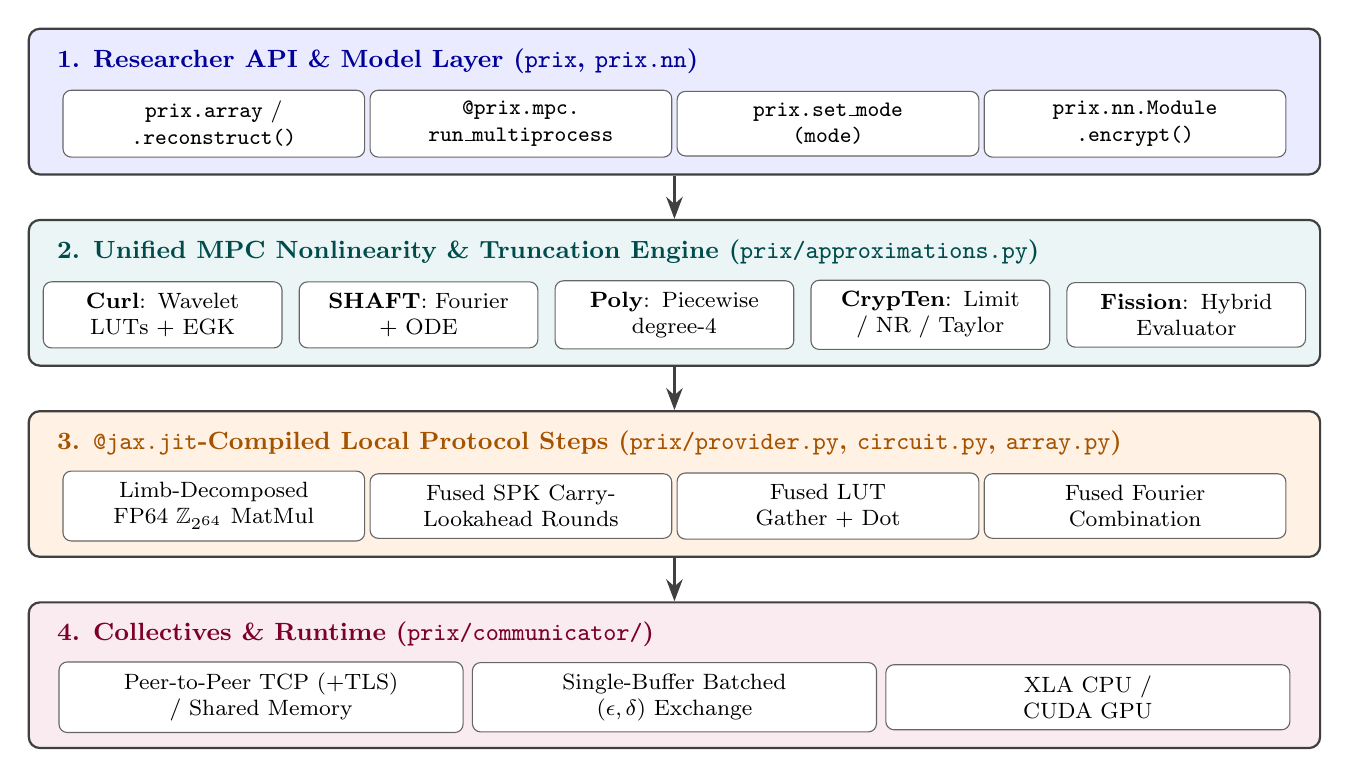
\begin{tikzpicture}[
    node distance=0.55cm,
    layer/.style={rectangle, rounded corners=4pt, draw=black!75, thick, minimum width=16.4cm, minimum height=1.85cm},
    subbox/.style={rectangle, rounded corners=3pt, draw=black!60, fill=white, text width=3.55cm, minimum height=0.82cm, inner sep=4pt, align=center, font=\footnotesize},
    subbox3/.style={rectangle, rounded corners=3pt, draw=black!60, fill=white, text width=4.85cm, minimum height=0.82cm, inner sep=4pt, align=center, font=\footnotesize},
    subbox5/.style={rectangle, rounded corners=3pt, draw=black!60, fill=white, text width=2.75cm, minimum height=0.82cm, inner sep=4pt, align=center, font=\footnotesize},
    arrow/.style={-{Stealth[length=2.8mm]}, thick, draw=black!75}
]
    % Layer 1: Researcher API
    \node[layer, fill=blue!8] (l1) {};
    \node[anchor=north west, font=\small\bfseries, text=blue!60!black] at ($(l1.north west)+(0.25,-0.14)$) {1. Researcher API \& Model Layer (\texttt{prix}, \texttt{prix.nn})};
    \node[subbox] at ($(l1.center)+(-5.85,-0.28)$) {\texttt{prix.array} /\\ \texttt{.reconstruct()}};
    \node[subbox] at ($(l1.center)+(-1.95,-0.28)$) {\texttt{@prix.mpc.}\\ \texttt{run\_multiprocess}};
    \node[subbox] at ($(l1.center)+(1.95,-0.28)$) {\texttt{prix.set\_mode}\\\texttt{(mode)}};
    \node[subbox] at ($(l1.center)+(5.85,-0.28)$) {\texttt{prix.nn.Module}\\ \texttt{.encrypt()}};

    % Layer 2: Unified Dispatch
    \node[layer, fill=teal!8, below=of l1] (l2) {};
    \node[anchor=north west, font=\small\bfseries, text=teal!60!black] at ($(l2.north west)+(0.25,-0.14)$) {2. Unified MPC Nonlinearity \& Truncation Engine (\texttt{prix/approximations.py})};
    \node[subbox5] at ($(l2.center)+(-6.5,-0.28)$) {\textbf{Curl}: Wavelet\\ LUTs + EGK};
    \node[subbox5] at ($(l2.center)+(-3.25,-0.28)$) {\textbf{SHAFT}: Fourier\\ + ODE};
    \node[subbox5] at ($(l2.center)+(0,-0.28)$) {\textbf{Poly}: Piecewise\\ degree-4};
    \node[subbox5] at ($(l2.center)+(3.25,-0.28)$) {\textbf{CrypTen}: Limit\\ / NR / Taylor};
    \node[subbox5] at ($(l2.center)+(6.5,-0.28)$) {\textbf{Fission}: Hybrid\\ Evaluator};

    % Layer 3: XLA Fused Kernels
    \node[layer, fill=orange!10, below=of l2] (l3) {};
    \node[anchor=north west, font=\small\bfseries, text=orange!65!black] at ($(l3.north west)+(0.25,-0.14)$) {3. \texttt{@jax.jit}-Compiled Local Protocol Steps (\texttt{prix/provider.py}, \texttt{circuit.py}, \texttt{array.py})};
    \node[subbox] at ($(l3.center)+(-5.85,-0.28)$) {Limb-Decomposed\\ FP64 $\Zring$ MatMul};
    \node[subbox] at ($(l3.center)+(-1.95,-0.28)$) {Fused SPK Carry-\\Lookahead Rounds};
    \node[subbox] at ($(l3.center)+(1.95,-0.28)$) {Fused LUT\\ Gather + Dot};
    \node[subbox] at ($(l3.center)+(5.85,-0.28)$) {Fused Fourier\\ Combination};

    % Layer 4: Collectives & Hardware
    \node[layer, fill=purple!8, below=of l3] (l4) {};
    \node[anchor=north west, font=\small\bfseries, text=purple!65!black] at ($(l4.north west)+(0.25,-0.14)$) {4. Collectives \& Runtime (\texttt{prix/communicator/})};
    \node[subbox3] at ($(l4.center)+(-5.25,-0.28)$) {Peer-to-Peer TCP (+TLS)\\ / Shared Memory};
    \node[subbox3] at ($(l4.center)+(0.0,-0.28)$) {Single-Buffer Batched\\ $(\epsilon, \delta)$ Exchange};
    \node[subbox3] at ($(l4.center)+(5.25,-0.28)$) {XLA CPU /\\ CUDA GPU};

    \draw[arrow] (l1.south) -- (l2.north);
    \draw[arrow] (l2.south) -- (l3.north);
    \draw[arrow] (l3.south) -- (l4.north);
\end{tikzpicture}%
}
\caption{System architecture of \textbf{PriX}, from the researcher-facing Python API down to compiled local protocol steps and transports.}
\label{fig:architecture}
\end{figure}

Figure~\ref{fig:architecture} presents the four-layer architecture of PriX. Eager PyTorch frameworks launch each ring-arithmetic or bitwise operation as its own kernel. PriX instead expresses the local (non-communicating) phase between two openings of a protocol as a pure function over 64-bit JAX arrays (\texttt{jnp.int64} / \texttt{jnp.uint64}) and compiles it with \texttt{@jax.jit}, so each such phase becomes one XLA executable. Communication remains on the host between compiled phases.

\subsection{Exact Limb-Decomposed FP64 Matrix Multiplication over $\Zring$}
\label{sec:limb_matmul}
Neither CPU BLAS libraries nor cuBLAS provide 64-bit integer (\texttt{int64}) GEMM, so PyTorch's \texttt{int64} matmul runs on generic unblocked loops. Double-precision GEMM, by contrast, is available in optimized form on both (AVX/FMA on CPU, \texttt{cublasDgemm} on GPU). Note that on the Tesla T4 used in our GPU experiments, FP64 throughput is a small fraction of FP32 throughput and does not use tensor cores.

To compute $C = A B \bmod 2^{64}$ for $A \in \Zring^{M \times K}$ and $B \in \Zring^{K \times N}$ exactly in FP64, we split each unsigned 64-bit entry into $L$ limbs of $w$ bits, $A = \sum_{i} A_i 2^{wi}$ and $B = \sum_j B_j 2^{wj}$. Because only the result modulo $2^{64}$ is needed, every limb pair with $(i + j)\,w \ge 64$ contributes a multiple of $2^{64}$ and can be skipped:
\begin{equation}
    A B \equiv \sum_{(i + j)\,w < 64} (A_i B_j) \, 2^{w(i + j)} \pmod{2^{64}}.
    \label{eq:ten_limbs}
\end{equation}
PriX uses two limb configurations, chosen by the contraction size $K$:
\begin{itemize}
    \item $K \le 512$: $L = 3$ limbs of $w = 22$ bits ($A_2, B_2$ have 20 bits), so only the \textbf{6} pairs with $i + j \le 2$ are computed. Each product entry is below $K \cdot 2^{44} \le 2^{53}$, so every FP64 GEMM is exact.
    \item $K > 512$: $L = 4$ limbs of $w = 16$ bits, so only the \textbf{10} pairs with $i + j \le 3$ are computed. On GPU each pair is a separate slice of one batched GEMM. Each pair product is converted to \texttt{uint64} individually, which is exact for $K \cdot 2^{32} \le 2^{53}$, i.e.\ $K \le 2^{21}$. On CPU, each pair product is likewise converted to \texttt{uint64} before products of equal shift are added, so both backends share the same $K \le 2^{21}$ bound.
    \item $K > 2^{21}$: the contraction is split into chunks of at most $2^{21}$. Each chunk is multiplied exactly as above, and the \texttt{uint64} partial results are added; wrap-around addition is exact modulo $2^{64}$, so the result is bit-exact for any $K$. The chunking is decided at trace time, so it adds no overhead when $K \le 2^{21}$.
\end{itemize}
CrypTen's CUDA backend~\cite{knott2021crypten} uses 3 limbs for $K < 256$ and 4 limbs otherwise, and computes \emph{all} $9$ or $16$ limb products in one batched \texttt{torch.matmul} before discarding the vanishing ones. PriX therefore performs 6 instead of 9 GEMMs for $K < 256$, 6 instead of 16 for $256 \le K \le 512$, and 10 instead of 16 for $K > 512$. On GPU, PriX stacks the surviving limb pairs into one batched GEMM, and the limb extraction, GEMM, conversion, shifts, and modular accumulation are compiled together with the Beaver combination $\shareA{C} + \epsilon \shareA{B} + \shareA{A}\delta + \mathbb{I}[p=0](\epsilon\delta)$. On CPU, CrypTen uses PyTorch's \texttt{int64} matmul directly, so PriX's advantage there comes mainly from using FP64 BLAS.

\subsection{Compiled Set-Propagate-Kill Comparison Circuits}
\label{sec:koggestone}
Private comparisons ($\shareA{x} < 0$, $\operatorname{ReLU}$, $\operatorname{Max}$) extract the most significant bit of a secret-shared ring element by converting $\shareA{x}$ into binary shares with a parallel-prefix carry-lookahead circuit. Like CrypTen, PriX uses a carry-lookahead adder built from set/propagate (Set-Propagate-Kill, SPK) carry signals~\cite{damgard2006unconditionally}, arranged as a Kogge--Stone parallel-prefix tree~\cite{kogge1973parallel} with $\log_2 64 = 6$ rounds. In round $r$ with stride $s = 2^r$, the set and propagate bit-vectors are updated as
\begin{equation}
    S^{(r+1)} = S^{(r)} \oplus \big(P^{(r)} \wedge (S^{(r)} \ll s)\big), \qquad
    P^{(r+1)} = P^{(r)} \wedge (P^{(r)} \ll s),
\end{equation}
where XOR can replace OR because the two terms are never both set. As in CrypTen, both AND gates of a round are opened in one batched binary-Beaver exchange. PriX differs in how the local work is executed:
\begin{itemize}
    \item The dealer generates the binary triples for all 6 rounds in one call (\texttt{generate\_spk\_triples}) instead of one call per round.
    \item The local work between two consecutive openings---applying the previous round's Beaver correction, masking, shifting, and preparing the next round's masked operands---is one compiled kernel (\texttt{\_spk\_step\_fused} in \texttt{circuit.py}). The first and last rounds are fused with the arithmetic-to-binary conversion and with the binary-to-arithmetic conversion of the sign bit, respectively (\texttt{\_a2b\_post\_and\_spk\_round0\_pre}, \texttt{\_spk\_round\_last\_and\_ltz\_b2a\_pre}, \texttt{\_b2a\_combine}).
\end{itemize}

\subsection{Compiled Wavelet LUT Evaluation and Fourier Combination}
\label{sec:lut_shaft_fusion}
In Curl mode (\texttt{mode="curl"}), a nonlinearity such as $\operatorname{InvSqrt}$, $\operatorname{Exp}$, $\operatorname{GeLU}$, or $\operatorname{SiLU}$ truncates the secret input to a table index, reveals the index masked by a one-hot correlation, rotates the one-hot share accordingly, and takes its dot product with the (Biorthogonal-2.2) coefficient tables before interpolating. In PriX:
\begin{itemize}
    \item Each wavelet table is built on first use, placed on the accelerator, and cached for the rest of the session (\texttt{LookupTables(device)}), so table construction is excluded from the timed runs by the warmup.
    \item The rotation and dot product against one table, or against the two Biorthogonal-2.2 tables used for interpolation, are one compiled kernel (\texttt{\_lut\_gather\_dot}, \texttt{\_bior\_lut\_gather\_dot} in \texttt{array.py}).
    \item In SHAFT mode, after the single opening of $\delta = x - t$, the evaluation of Equation~\ref{eq:shaft_trig} for all $K$ terms---computing $\sin(k\omega\delta)$ and $\cos(k\omega\delta)$, scaling them by $\beta_k$, multiplying against the triple shares, and summing---is one compiled kernel (\texttt{\_fourier\_linear\_comb\_jit} in \texttt{approximations.py}).
\end{itemize}

\subsection{Batched Openings and Transports}
\label{sec:collectives}
Every private multiplication opens two masked tensors, $\epsilon = x - a$ and $\delta = y - b$. As in CrypTen, both are opened in one round. When $\epsilon$ and $\delta$ have different shapes (e.g.\ $\epsilon \in \Zring^{M \times K}$ and $\delta \in \Zring^{K \times N}$ in a matrix multiplication), PriX passes both to one batched \texttt{all\_reduce}, which sends them as a single message and splits the result.

PriX's default transport is \textbf{peer-to-peer TCP}: every pair of processes (MPC parties, the TTP dealer if used, and Fission evaluators) shares one direct connection, with no coordinator in the data path, and the same code runs on one host over loopback or across machines. Messages use a small binary format that carries only plain data and numeric arrays, so, unlike pickle, decoding a malicious peer's message cannot execute code. Sockets are non-blocking, and every wait keeps flushing queued outgoing data, so two parties that send each other large openings at the same time cannot deadlock. Connections can optionally use mutual TLS with a shared certificate authority; all experiments here run without TLS, like CrypTen's transport. For single-host simulation, PriX also offers a \textbf{shared-memory transport}: a 4-slot ring buffer (\texttt{multiprocessing.RawArray}) per party with a 1-byte pipe message as the readiness signal, with slots of $2^{21}$ \texttt{int64} values (16\,MiB) and a pickled-queue fallback for larger openings. CrypTen uses \texttt{torch.distributed} with the \texttt{gloo} backend over loopback TCP. Section~\ref{sec:ablation} compares all three.

%======================================================================
\section{Researcher Ergonomics and Unified API}
\label{sec:api}
%======================================================================

A central design goal of PriX is enabling cryptography and machine learning researchers to prototype and benchmark private Transformer protocols with minimal boilerplate. Listing~\ref{lst:quickstart} shows a multi-party ablation that evaluates a pre-norm Transformer block under all five approximation modes.

\begin{lstlisting}[style=pythonstyle, caption={Evaluating a private Transformer block under all five MPC approximation modes in PriX.}, label={lst:quickstart}]
import numpy as np
import prix
import prix.nn as nn

class TransformerBlock(nn.Module):
    def __init__(self, d_model=64, n_heads=4, d_ff=256):
        super().__init__()
        self.ln1 = nn.LayerNorm(d_model)
        self.attn = nn.MultiheadAttention(d_model, n_heads)
        self.ln2 = nn.LayerNorm(d_model)
        self.ffn = nn.Sequential(nn.Linear(d_model, d_ff), nn.GELU(), nn.Linear(d_ff, d_model))

    def forward(self, x):
        h = self.ln1(x)
        x = x + self.attn(h, h, h)
        return x + self.ffn(self.ln2(x))

def evaluate_private_block(tokens):
    # Party 0 secret-shares the model weights; party 1 secret-shares the token embeddings
    model = TransformerBlock().encrypt(src=0)
    x = prix.array(tokens, src=1)
    return model(x).reconstruct()

tokens = np.random.randn(1, 16, 64).astype(np.float32)
for mode in ["crypten", "poly", "shaft", "curl", "fission"]:
    out = prix.run(evaluate_private_block, tokens, world_size=2, mode=mode)
\end{lstlisting}

%======================================================================
\section{Experimental Evaluation}
\label{sec:evaluation}
%======================================================================

\subsection{Experimental Setup}
We compare \textbf{PriX (JAX)} against a PyTorch \textbf{CrypTen} baseline~\cite{knott2021crypten}: the CrypTen fork that serves as the reference implementation of Curl~\cite{santos2024curl} and Fission~\cite{ugurbil2025fission}. SHAFT's Fourier activations and ODE Softmax~\cite{kei2025shaft}, and the piecewise polynomials of \texttt{poly} mode, are added to this baseline by our benchmark script. The SHAFT functions follow the SHAFT authors' CrypTen-based reference implementation, which computes $\operatorname{GeLU}$/$\operatorname{SiLU}$ with $\operatorname{ReLU}$ followed by a separate range comparison. PUMA, BOLT, and Nimbus have no CrypTen implementation, so the \texttt{poly} functions are ports of PriX's algorithms with the same coefficients, intervals, batched comparisons, and power-basis sharing. Where PriX seeds Newton--Raphson iterations with the limit approximation of $\exp$ regardless of the configured $\exp$ method, the baseline is configured the same way. Both frameworks run 2-party semi-honest protocols with the Trusted First Party (\texttt{TFP}) dealer, $f = 16$ fractional bits, identical inputs, and identical configurations: each mode's YAML is merged over the framework's default configuration, and the CrypTen side then takes PriX's value for every setting both define, including the adjusted LUT ranges of Section~\ref{sec:accuracy} (a configuration change only; the baseline code is unchanged). The five modes are:
\begin{enumerate}
    \item \textbf{CrypTen approximations (\texttt{crypten})}~\cite{knott2021crypten};
    \item \textbf{Piecewise polynomials (\texttt{poly})}~\cite{dong2023puma,pang2024bolt,li2024nimbus};
    \item \textbf{SHAFT Fourier + ODE (\texttt{shaft})}~\cite{kei2025shaft};
    \item \textbf{Curl wavelet LUTs with $\mathsf{TruncPr}$ (\texttt{curl})}~\cite{santos2024curl}; and
    \item \textbf{Fission hybrid evaluator (\texttt{fission})}~\cite{ugurbil2025fission}, with one evaluator process.
\end{enumerate}
We benchmark 10 MPC primitives and nonlinearities ($\text{MatMul } 128\times 128$, $\text{Mul } 128\times 128$, $\text{ReLU } 32\times 64$, $\text{Exp } 32\times 64$, $\text{Reciprocal } 32\times 64$, $\text{InvSqrt } 32\times 64$, $\text{GeLU } 32\times 64$, $\text{SiLU } 32\times 64$, $\text{Softmax } 4\times 32\times 32$, $\text{LayerNorm } 4\times 32\times 64$) and 5 Transformer configurations with sequence length $L=16$: \texttt{BertTiny} (2 blocks, $d=128$, $H=2$), \texttt{BertBase} (1 block, $d=768$, $H=12$), \texttt{GPT2} (1 block, $d=768$, $H=12$), \texttt{Llama} (1 block, $d=768$, $H=12$, $H_{\text{kv}}=4$, RoPE + SwiGLU + RMSNorm, grouped-query attention), and \texttt{ModernBert} (1 block, $d=768$, $H=12$, RoPE + GeGLU). Weights and inputs are random; we measure latency only, not model accuracy.

\paragraph{Methodology.} All parties run as separate processes on one host and communicate over loopback TCP: CrypTen through \texttt{torch.distributed}/\texttt{gloo}, and PriX through its own peer-to-peer TCP transport (Section~\ref{sec:collectives}), without TLS in either case. No network latency or bandwidth limit is emulated. Each primitive is run 2 times untimed (to exclude JIT compilation and cache warmup) and then timed 5 times; each Transformer block is warmed up once and timed 3 times. Parties synchronize with a barrier before every timed run, device work is synchronized before the timer stops, and we report the median. Communication statistics (rounds and bytes) were recorded in all runs. On each platform, all configurations (CrypTen, and PriX over each of its three transports; Section~\ref{sec:ablation}) were measured in one session (on CPU, rotating the order of the four runs between modes so that slow drift of the host does not favor one of them). CPU experiments use the host listed in Table~\ref{tab:cpu_llm}'s caption. GPU experiments use a Google Colab instance with one NVIDIA Tesla T4. With so few repetitions, differences of roughly 10\% or less between the two frameworks should be treated as within run-to-run noise.

\begin{figure}[t]
\centering
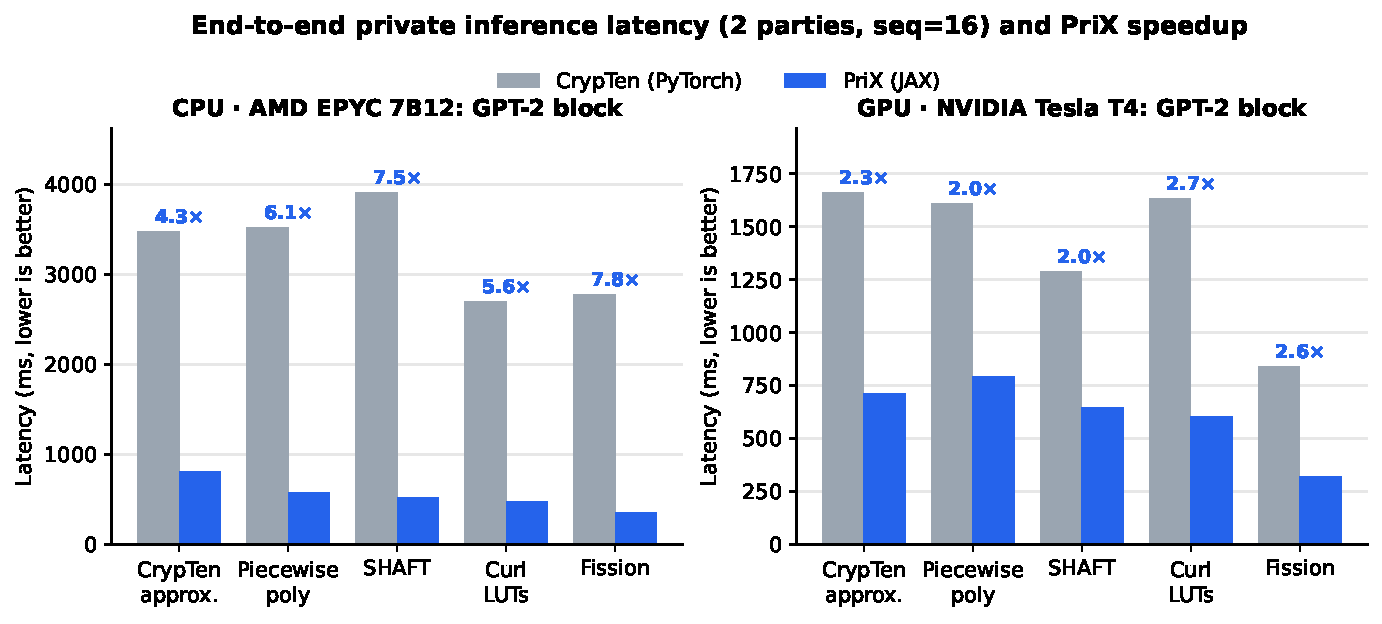
\includegraphics[width=\textwidth]{figures/llm_latency.pdf}
\caption{End-to-end latency of one GPT-2 block ($d=768$, $L=16$, 2 parties) for CrypTen and PriX under each approximation mode, on CPU (left) and GPU (right). Labels give the PriX speedup.}
\label{fig:llm_latency}
\end{figure}

\begin{figure}[t]
\centering
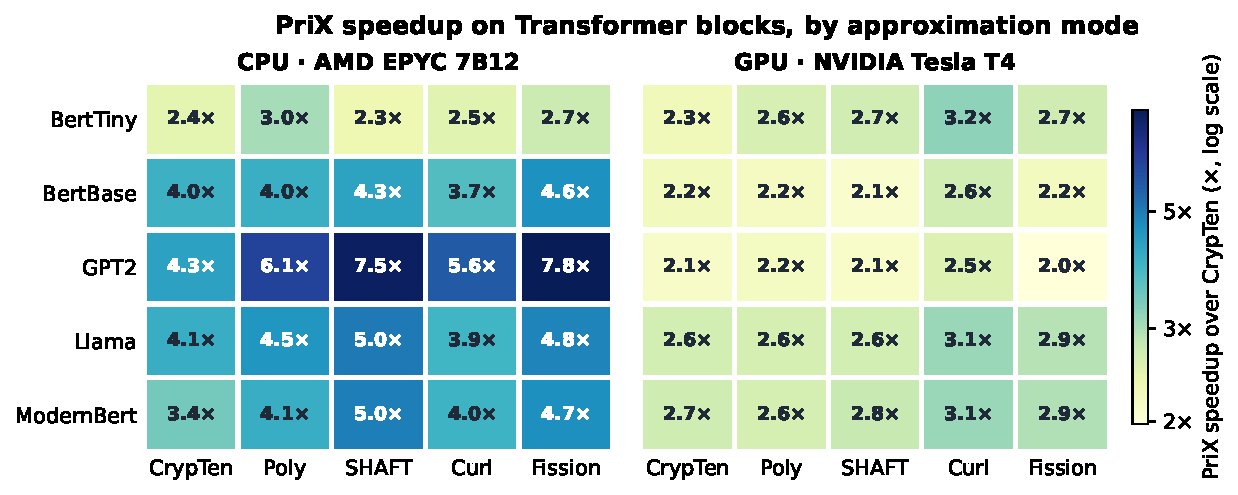
\includegraphics[width=\textwidth]{figures/llm_speedup.pdf}
\caption{PriX speedup over CrypTen on all five Transformer blocks and all five approximation modes, on CPU and GPU (log color scale). The CrypTen \texttt{fission} column on CPU is affected by contention from the evaluator process (Section~\ref{sec:evaluation}).}
\label{fig:llm_speedup}
\end{figure}

\begin{figure}[t]
\centering
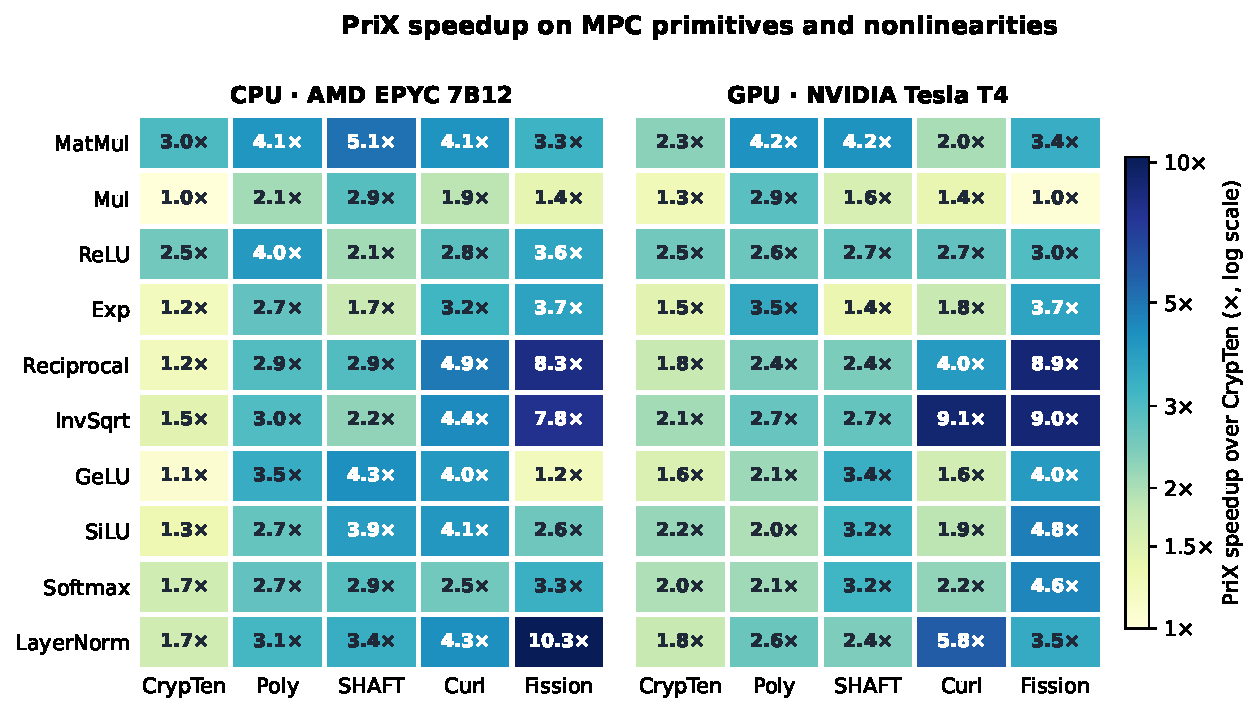
\includegraphics[width=\textwidth]{figures/primitive_speedup.pdf}
\caption{PriX speedup over CrypTen on the 10 MPC primitives and nonlinearities, on CPU and GPU (log color scale).}
\label{fig:primitive_speedup}
\end{figure}

Figures~\ref{fig:llm_latency}--\ref{fig:primitive_speedup} summarize the results; Tables~\ref{tab:cpu_llm}--\ref{tab:gpu_ops} give the underlying numbers.

\subsection{CPU Benchmarks}

\begin{table}[t]
\centering
\caption{\textbf{CPU Transformer-block latency (ms) and PriX speedup} for all five approximation modes ($N=2$ parties, $L=16$; median of 3 timed runs). Host: AMD EPYC 7B12, 24 vCPUs; Python 3.13, JAX/jaxlib 0.12.0, PyTorch 2.14.1 (CPU). PriX uses its default peer-to-peer TCP transport; CrypTen uses \texttt{gloo} over TCP. All entries were measured in one session. Lower is better.}
\label{tab:cpu_llm}
\vspace{2pt}
\resizebox{\textwidth}{!}{%
\begin{tabular}{@{}lrrrrrrrrrr@{}}
\toprule
& \multicolumn{2}{c}{\textbf{CrypTen Approx.}} & \multicolumn{2}{c}{\textbf{Piecewise Poly}} & \multicolumn{2}{c}{\textbf{SHAFT (Fourier+ODE)}} & \multicolumn{2}{c}{\textbf{Curl Wavelet LUTs}} & \multicolumn{2}{c}{\textbf{Fission Evaluator}} \\
\cmidrule(lr){2-3} \cmidrule(lr){4-5} \cmidrule(lr){6-7} \cmidrule(lr){8-9} \cmidrule(lr){10-11}
\textbf{Model} & CrypTen & \textbf{PriX (Speedup)} & CrypTen & \textbf{PriX (Speedup)} & CrypTen & \textbf{PriX (Speedup)} & CrypTen & \textbf{PriX (Speedup)} & CrypTen & \textbf{PriX (Speedup)} \\
\midrule
BertTiny (2-Blk)   & 1423.31 & \textbf{582.27 (2.44$\times$)} & 1687.14 & \textbf{560.17 (3.01$\times$)} & 1010.66 & \textbf{434.93 (2.32$\times$)} & 1106.85 & \textbf{446.87 (2.48$\times$)} & 443.46 & \textbf{163.33 (2.72$\times$)} \\
BertBase (1-Blk)   & 2950.74 & \textbf{737.85 (4.00$\times$)} & 2968.03 & \textbf{733.66 (4.05$\times$)} & 3154.52 & \textbf{735.38 (4.29$\times$)} & 2167.78 & \textbf{582.69 (3.72$\times$)} & 2081.62 & \textbf{449.65 (4.63$\times$)} \\
GPT2 (1-Blk)       & 3480.96 & \textbf{809.60 (4.30$\times$)} & 3524.84 & \textbf{574.84 (6.13$\times$)} & 3915.11 & \textbf{519.49 (7.54$\times$)} & 2702.19 & \textbf{482.07 (5.61$\times$)} & 2776.97 & \textbf{357.22 (7.77$\times$)} \\
Llama (1-Blk)      & 2317.26 & \textbf{566.54 (4.09$\times$)} & 2779.46 & \textbf{612.08 (4.54$\times$)} & 3021.76 & \textbf{600.14 (5.04$\times$)} & 2068.08 & \textbf{525.26 (3.94$\times$)} & 2244.43 & \textbf{463.35 (4.84$\times$)} \\
ModernBert (1-Blk) & 1899.87 & \textbf{557.62 (3.41$\times$)} & 2099.36 & \textbf{514.43 (4.08$\times$)} & 2236.08 & \textbf{450.99 (4.96$\times$)} & 1685.12 & \textbf{425.10 (3.96$\times$)} & 1432.81 & \textbf{307.39 (4.66$\times$)} \\
\bottomrule
\end{tabular}%
}
\end{table}

\begin{table}[t]
\centering
\caption{\textbf{CPU primitive and nonlinearity latency (ms, CrypTen / PriX)} and PriX speedup (median of 5 timed runs; same host and session as Table~\ref{tab:cpu_llm}).}
\label{tab:cpu_ops}
\vspace{2pt}
\resizebox{\textwidth}{!}{%
\begin{tabular}{@{}lrrrrr@{}}
\toprule
\textbf{Operation (Shape)} & \textbf{CrypTen Approx.} & \textbf{Piecewise Poly} & \textbf{SHAFT (Fourier+ODE)} & \textbf{Curl Wavelet LUTs} & \textbf{Fission Evaluator} \\
\midrule
Private MatMul ($128\times 128$)   & 23.89 / \textbf{5.82 (4.10$\times$)} & 24.54 / \textbf{6.55 (3.75$\times$)} & 25.05 / \textbf{6.15 (4.08$\times$)} & 28.34 / \textbf{7.49 (3.78$\times$)} & 29.61 / \textbf{7.70 (3.84$\times$)} \\
Private Mul ($128\times 128$)      & 5.29 / \textbf{4.95 (1.07$\times$)} & 5.89 / \textbf{3.65 (1.61$\times$)} & 4.85 / \textbf{4.57 (1.06$\times$)} & 9.48 / \textbf{6.39 (1.48$\times$)} & 6.90 / \textbf{4.47 (1.54$\times$)} \\
Comparison / ReLU ($32\times 64$)  & 32.52 / \textbf{9.46 (3.44$\times$)} & 36.94 / \textbf{9.50 (3.89$\times$)} & 31.10 / \textbf{10.06 (3.09$\times$)} & 30.12 / \textbf{13.09 (2.30$\times$)} & 41.98 / \textbf{13.25 (3.17$\times$)} \\
Exp ($32\times 64$)                & 21.08 / \textbf{14.97 (1.41$\times$)} & 52.61 / \textbf{19.06 (2.76$\times$)} & 20.77 / \textbf{17.73 (1.17$\times$)} & 68.19 / \textbf{14.94 (4.56$\times$)} & 10.90 / \textbf{2.67 (4.08$\times$)} \\
Reciprocal ($32\times 64$)         & 105.89 / \textbf{49.65 (2.13$\times$)} & 128.86 / \textbf{40.38 (3.19$\times$)} & 95.99 / \textbf{59.46 (1.61$\times$)} & 50.35 / \textbf{9.53 (5.29$\times$)} & 19.56 / \textbf{2.67 (7.33$\times$)} \\
InvSqrt ($32\times 64$)            & 65.45 / \textbf{34.43 (1.90$\times$)} & 67.89 / \textbf{31.04 (2.19$\times$)} & 69.75 / \textbf{45.42 (1.54$\times$)} & 122.58 / \textbf{19.72 (6.22$\times$)} & 20.26 / \textbf{1.53 (13.25$\times$)} \\
GeLU ($32\times 64$)               & 114.98 / \textbf{62.66 (1.83$\times$)} & 59.24 / \textbf{24.05 (2.46$\times$)} & 83.85 / \textbf{24.27 (3.45$\times$)} & 34.11 / \textbf{8.18 (4.17$\times$)} & 11.13 / \textbf{2.60 (4.29$\times$)} \\
SiLU ($32\times 64$)               & 83.53 / \textbf{39.35 (2.12$\times$)} & 53.84 / \textbf{23.47 (2.29$\times$)} & 74.87 / \textbf{34.21 (2.19$\times$)} & 35.45 / \textbf{7.40 (4.79$\times$)} & 12.00 / \textbf{1.80 (6.68$\times$)} \\
Softmax ($4\times 32\times 32$)    & 382.48 / \textbf{169.38 (2.26$\times$)} & 442.88 / \textbf{159.95 (2.77$\times$)} & 178.78 / \textbf{136.92 (1.31$\times$)} & 378.89 / \textbf{120.87 (3.13$\times$)} & 18.56 / \textbf{2.87 (6.46$\times$)} \\
LayerNorm ($4\times 32\times 64$)  & 75.40 / \textbf{28.37 (2.66$\times$)} & 72.25 / \textbf{31.84 (2.27$\times$)} & 76.07 / \textbf{40.36 (1.88$\times$)} & 55.58 / \textbf{13.91 (4.00$\times$)} & 21.72 / \textbf{3.07 (7.07$\times$)} \\
\bottomrule
\end{tabular}%
}
\end{table}

Tables~\ref{tab:cpu_llm} and~\ref{tab:cpu_ops} report the CPU results. PriX has lower latency than CrypTen in all 75 CPU configurations: Transformer-block speedups range from \textbf{2.32$\times$} to \textbf{7.77$\times$} (geometric mean 4.14$\times$), and primitive speedups from 1.06$\times$ (Mul, \texttt{shaft} mode) to 13.25$\times$ (InvSqrt, \texttt{fission} mode).
\begin{itemize}
    \item \textbf{Run-to-run noise.} ReLU has the same protocol in every mode, so its spread across modes gives a rough noise estimate. Within this session, CrypTen's ReLU took 30.1--36.9\,ms in four modes and 42.0\,ms in \texttt{fission} mode, where an extra evaluator process competes for the same host; PriX's took 9.5--13.3\,ms. Single-operation speedups below about 1.2$\times$ (Mul in \texttt{crypten} and \texttt{shaft} modes, Exp in \texttt{shaft} mode) are within this noise. The host is a shared cloud VM, and absolute latencies vary between sessions: both frameworks ran about 25--40\% slower (median) in this session than in an earlier one with the same software. Only comparisons within one session are meaningful, which is why all CPU numbers in this paper come from a single session.
    \item \textbf{Matrix multiplication.} On CPU, CrypTen uses PyTorch's \texttt{int64} matmul, which has no BLAS backend. PriX uses FP64 GEMM on limbs (Section~\ref{sec:limb_matmul}), which explains the 3.8--4.1$\times$ MatMul speedups in every mode. Linear layers dominate the $d = 768$ blocks, which is consistent with their larger end-to-end speedups (3.4--7.8$\times$) compared with \texttt{BertTiny} (2.3--3.0$\times$).
    \item \textbf{Comparisons and LUTs.} ReLU is 2.3--3.9$\times$ faster, consistent with fusing the local work of each SPK round and with its 20\% smaller openings (Section~\ref{sec:ablation}). In \texttt{curl} mode, InvSqrt drops from 122.6 to 19.7\,ms (6.22$\times$), SiLU from 35.5 to 7.4\,ms (4.79$\times$), and LayerNorm from 55.6 to 13.9\,ms (4.00$\times$).
    \item \textbf{Piecewise polynomials.} \texttt{poly} mode makes GeLU and SiLU cheaper than \texttt{crypten} mode in both frameworks (in PriX, 24.1 vs.\ 62.7\,ms and 23.5 vs.\ 39.4\,ms), but more expensive than Curl's LUTs (8.2 and 7.4\,ms). For $\exp$, the piecewise polynomial is \emph{slower} than the limit approximation (19.1 vs.\ 15.0\,ms in PriX) because its secure comparisons cost more than 8 squarings.
\end{itemize}

\subsection{GPU Benchmarks (NVIDIA Tesla T4, CUDA)}

\begin{table}[t]
\centering
\caption{\textbf{GPU (NVIDIA Tesla T4, Google Colab) Transformer-block latency (ms) and PriX speedup} for all five approximation modes ($N=2$ parties, $L=16$; median of 3 timed runs). PriX uses its default peer-to-peer TCP transport; CrypTen uses \texttt{gloo} over TCP. All entries were measured in one session. Lower is better.}
\label{tab:gpu_llm}
\vspace{2pt}
\resizebox{\textwidth}{!}{%
\begin{tabular}{@{}lrrrrrrrrrr@{}}
\toprule
& \multicolumn{2}{c}{\textbf{CrypTen Approx.}} & \multicolumn{2}{c}{\textbf{Piecewise Poly}} & \multicolumn{2}{c}{\textbf{SHAFT (Fourier+ODE)}} & \multicolumn{2}{c}{\textbf{Curl Wavelet LUTs}} & \multicolumn{2}{c}{\textbf{Fission Evaluator}} \\
\cmidrule(lr){2-3} \cmidrule(lr){4-5} \cmidrule(lr){6-7} \cmidrule(lr){8-9} \cmidrule(lr){10-11}
\textbf{Model} & CrypTen & \textbf{PriX (Speedup)} & CrypTen & \textbf{PriX (Speedup)} & CrypTen & \textbf{PriX (Speedup)} & CrypTen & \textbf{PriX (Speedup)} & CrypTen & \textbf{PriX (Speedup)} \\
\midrule
BertTiny (2-Blk)   & 1935.00 & \textbf{867.19 (2.23$\times$)} & 1815.61 & \textbf{826.13 (2.20$\times$)} & 1197.88 & \textbf{537.35 (2.23$\times$)} & 1968.48 & \textbf{639.19 (3.08$\times$)} & 396.46 & \textbf{155.38 (2.55$\times$)} \\
BertBase (1-Blk)   & 1662.57 & \textbf{761.04 (2.18$\times$)} & 1676.78 & \textbf{763.90 (2.20$\times$)} & 1321.44 & \textbf{650.66 (2.03$\times$)} & 1694.65 & \textbf{600.76 (2.82$\times$)} & 926.40 & \textbf{350.81 (2.64$\times$)} \\
GPT2 (1-Blk)       & 1663.77 & \textbf{712.28 (2.34$\times$)} & 1609.94 & \textbf{794.24 (2.03$\times$)} & 1290.56 & \textbf{645.33 (2.00$\times$)} & 1634.65 & \textbf{604.11 (2.71$\times$)} & 838.81 & \textbf{320.92 (2.61$\times$)} \\
Llama (1-Blk)      & 1632.13 & \textbf{739.13 (2.21$\times$)} & 1580.11 & \textbf{729.44 (2.17$\times$)} & 1286.35 & \textbf{603.96 (2.13$\times$)} & 1728.45 & \textbf{658.25 (2.63$\times$)} & 983.09 & \textbf{402.74 (2.44$\times$)} \\
ModernBert (1-Blk) & 1445.26 & \textbf{686.65 (2.10$\times$)} & 1390.71 & \textbf{628.84 (2.21$\times$)} & 1085.58 & \textbf{568.86 (1.91$\times$)} & 1480.95 & \textbf{531.07 (2.79$\times$)} & 689.95 & \textbf{297.91 (2.32$\times$)} \\
\bottomrule
\end{tabular}%
}
\end{table}

\begin{table}[t]
\centering
\caption{\textbf{GPU (NVIDIA Tesla T4) primitive and nonlinearity latency (ms, CrypTen / PriX)} and PriX speedup (median of 5 timed runs; same session as Table~\ref{tab:gpu_llm}).}
\label{tab:gpu_ops}
\vspace{2pt}
\resizebox{\textwidth}{!}{%
\begin{tabular}{@{}lrrrrr@{}}
\toprule
\textbf{Operation (Shape)} & \textbf{CrypTen Approx.} & \textbf{Piecewise Poly} & \textbf{SHAFT (Fourier+ODE)} & \textbf{Curl Wavelet LUTs} & \textbf{Fission Evaluator} \\
\midrule
Private MatMul ($128\times 128$)   & 11.45 / \textbf{4.35 (2.63$\times$)} & 12.66 / \textbf{3.07 (4.12$\times$)} & 11.87 / \textbf{3.61 (3.29$\times$)} & 16.47 / \textbf{7.71 (2.14$\times$)} & 11.13 / \textbf{3.64 (3.05$\times$)} \\
Private Mul ($128\times 128$)      & 4.91 / \textbf{3.23 (1.52$\times$)} & 4.51 / \textbf{3.12 (1.45$\times$)} & 4.08 / \textbf{3.31 (1.23$\times$)} & 8.59 / \textbf{5.42 (1.59$\times$)} & 4.99 / \textbf{2.89 (1.73$\times$)} \\
Comparison / ReLU ($32\times 64$)  & 50.43 / \textbf{15.73 (3.21$\times$)} & 44.18 / \textbf{15.18 (2.91$\times$)} & 41.51 / \textbf{15.77 (2.63$\times$)} & 40.80 / \textbf{14.97 (2.73$\times$)} & 45.86 / \textbf{15.65 (2.93$\times$)} \\
Exp ($32\times 64$)                & 28.30 / \textbf{19.07 (1.48$\times$)} & 79.72 / \textbf{31.14 (2.56$\times$)} & 27.03 / \textbf{17.71 (1.53$\times$)} & 67.40 / \textbf{28.30 (2.38$\times$)} & 6.85 / \textbf{1.97 (3.49$\times$)} \\
Reciprocal ($32\times 64$)         & 129.92 / \textbf{65.24 (1.99$\times$)} & 134.66 / \textbf{68.01 (1.98$\times$)} & 137.68 / \textbf{69.79 (1.97$\times$)} & 56.21 / \textbf{12.59 (4.47$\times$)} & 17.61 / \textbf{1.48 (11.87$\times$)} \\
InvSqrt ($32\times 64$)            & 90.38 / \textbf{39.73 (2.28$\times$)} & 87.97 / \textbf{38.64 (2.28$\times$)} & 85.92 / \textbf{40.36 (2.13$\times$)} & 141.19 / \textbf{12.20 (11.57$\times$)} & 17.45 / \textbf{1.52 (11.49$\times$)} \\
GeLU ($32\times 64$)               & 150.42 / \textbf{73.75 (2.04$\times$)} & 68.45 / \textbf{37.10 (1.84$\times$)} & 92.71 / \textbf{29.91 (3.10$\times$)} & 23.39 / \textbf{12.35 (1.89$\times$)} & 6.81 / \textbf{1.71 (3.98$\times$)} \\
SiLU ($32\times 64$)               & 132.88 / \textbf{50.49 (2.63$\times$)} & 67.45 / \textbf{36.06 (1.87$\times$)} & 90.73 / \textbf{27.87 (3.26$\times$)} & 26.20 / \textbf{12.55 (2.09$\times$)} & 7.30 / \textbf{1.71 (4.26$\times$)} \\
Softmax ($4\times 32\times 32$)    & 551.32 / \textbf{251.27 (2.19$\times$)} & 586.34 / \textbf{252.38 (2.32$\times$)} & 199.67 / \textbf{106.15 (1.88$\times$)} & 507.15 / \textbf{200.35 (2.53$\times$)} & 7.23 / \textbf{1.74 (4.15$\times$)} \\
LayerNorm ($4\times 32\times 64$)  & 103.48 / \textbf{43.67 (2.37$\times$)} & 103.03 / \textbf{47.66 (2.16$\times$)} & 99.32 / \textbf{49.61 (2.00$\times$)} & 158.90 / \textbf{24.92 (6.38$\times$)} & 9.46 / \textbf{2.48 (3.81$\times$)} \\
\bottomrule
\end{tabular}%
}
\end{table}

Tables~\ref{tab:gpu_llm} and~\ref{tab:gpu_ops} report the GPU results. PriX has lower latency in all 75 GPU configurations, with Transformer-block speedups of \textbf{1.91$\times$--3.08$\times$} (geometric mean 2.33$\times$) and primitive speedups from 1.23$\times$ (Mul, \texttt{shaft} mode) to 11.87$\times$ (Reciprocal, \texttt{fission} mode).
\begin{itemize}
    \item \textbf{Run-to-run noise.} CrypTen's ReLU took 40.8--50.4\,ms across the five modes; PriX's took 15.0--15.8\,ms. PriX's MatMul was slower in \texttt{curl} mode (7.7\,ms vs.\ 3.1--4.4\,ms), where products use $\mathsf{TruncPr}$ rather than the communication-free local shift.
    \item \textbf{Comparisons.} CrypTen's ReLU on the GPU (41--50\,ms) is slower than on CPU, consistent with many small kernel launches per SPK round. PriX takes 15.0--15.8\,ms, a 2.6--3.2$\times$ speedup.
    \item \textbf{Wavelet LUTs.} In \texttt{curl} mode, InvSqrt drops from 141.2 to 12.2\,ms (11.57$\times$) and LayerNorm from 158.9 to 24.9\,ms (6.38$\times$). Both frameworks use the same Biorthogonal-2.2 configuration (one interval with a pair of slope/intercept tables). The gain comes from executing the same protocol with fewer launches and a faster local transport, not from a different algorithm.
    \item \textbf{SHAFT and piecewise polynomials.} Fourier GeLU drops from 92.7 to 29.9\,ms (3.10$\times$) and ODE Softmax from 199.7 to 106.2\,ms (1.88$\times$). Piecewise-polynomial GeLU and SiLU take 36--37\,ms in PriX, between SHAFT (28--30\,ms) and the \texttt{crypten} approximations (50--74\,ms). As on CPU, the piecewise $\exp$ is slower than the limit approximation (31.1 vs.\ 19.1\,ms).
    \item \textbf{End-to-end.} Transformer-block speedups are smaller on GPU (1.91--3.08$\times$) than on CPU. Plausible causes are the T4's low FP64 throughput and host-side communication, which faster GPU kernels do not reduce. We have not profiled this split.
\end{itemize}

\subsection{Transport Comparison: How Much Does the Transport Matter?}
\label{sec:ablation}
CrypTen and PriX use different transports (Section~\ref{sec:collectives}), so the speedups above combine PriX's compiled local computation with differences in how messages are moved. To separate the two, we ran PriX over each of its three transports in the same sessions as Tables~\ref{tab:cpu_llm}--\ref{tab:gpu_ops}: its default peer-to-peer TCP transport (the configuration in those tables); \texttt{torch.distributed}/\texttt{gloo} over TCP, i.e.\ CrypTen's own transport, by routing PriX's two-party \texttt{all\_reduce} through it; and the shared-memory transport. Everything else in PriX (compiled kernels, limb matrix multiplication, batching, host staging) is unchanged, and all three variants produce the same results. Table~\ref{tab:ablation} and Figure~\ref{fig:ablation} summarize the results as geometric means.

\begin{table}[t]
\centering
\caption{\textbf{PriX speedup over CrypTen by PriX transport, on CPU and GPU} (geometric means over the 5 Transformer blocks or the 10 primitives of each mode; same sessions as Tables~\ref{tab:cpu_llm} and~\ref{tab:gpu_llm}). CrypTen always uses \texttt{gloo} over TCP. ``gloo'' runs PriX over that same transport.}
\label{tab:ablation}
\vspace{2pt}
\footnotesize
\begin{tabular}{@{}lrrrrrr@{}}
\toprule
& \multicolumn{3}{c}{\textbf{Transformer blocks}} & \multicolumn{3}{c}{\textbf{Primitives}} \\
\cmidrule(lr){2-4} \cmidrule(lr){5-7}
\textbf{Platform / Mode} & TCP (default) & gloo & Shared mem. & TCP (default) & gloo & Shared mem. \\
\midrule
\multicolumn{7}{@{}l}{\emph{CPU (AMD EPYC 7B12)}} \\
CrypTen approx.  & 3.58$\times$ & 2.50$\times$ & 3.76$\times$ & 2.14$\times$ & 1.35$\times$ & 2.88$\times$ \\
Piecewise poly   & 4.25$\times$ & 3.21$\times$ & 4.98$\times$ & 2.63$\times$ & 1.59$\times$ & 3.08$\times$ \\
SHAFT            & 4.51$\times$ & 3.73$\times$ & 5.22$\times$ & 1.93$\times$ & 1.48$\times$ & 2.89$\times$ \\
Curl LUTs        & 3.81$\times$ & 2.77$\times$ & 3.35$\times$ & 3.70$\times$ & 2.05$\times$ & 4.13$\times$ \\
Fission          & 4.66$\times$ & 3.71$\times$ & 4.52$\times$ & 5.00$\times$ & 3.97$\times$ & 5.17$\times$ \\
\textbf{All modes (CPU)} & \textbf{4.14$\times$} & \textbf{3.14$\times$} & \textbf{4.31$\times$} & \textbf{2.89$\times$} & \textbf{1.92$\times$} & \textbf{3.53$\times$} \\
\midrule
\multicolumn{7}{@{}l}{\emph{GPU (NVIDIA Tesla T4)}} \\
CrypTen approx.  & 2.21$\times$ & 1.96$\times$ & 2.32$\times$ & 2.18$\times$ & 1.74$\times$ & 2.33$\times$ \\
Piecewise poly   & 2.16$\times$ & 1.94$\times$ & 2.33$\times$ & 2.26$\times$ & 1.77$\times$ & 2.37$\times$ \\
SHAFT            & 2.06$\times$ & 2.08$\times$ & 2.35$\times$ & 2.19$\times$ & 1.75$\times$ & 2.45$\times$ \\
Curl LUTs        & 2.80$\times$ & 2.47$\times$ & 2.87$\times$ & 3.06$\times$ & 2.35$\times$ & 3.07$\times$ \\
Fission          & 2.51$\times$ & 2.46$\times$ & 2.47$\times$ & 4.26$\times$ & 3.84$\times$ & 4.54$\times$ \\
\textbf{All modes (GPU)} & \textbf{2.33$\times$} & \textbf{2.17$\times$} & \textbf{2.46$\times$} & \textbf{2.69$\times$} & \textbf{2.17$\times$} & \textbf{2.85$\times$} \\
\bottomrule
\end{tabular}
\end{table}

\begin{figure}[t]
\centering
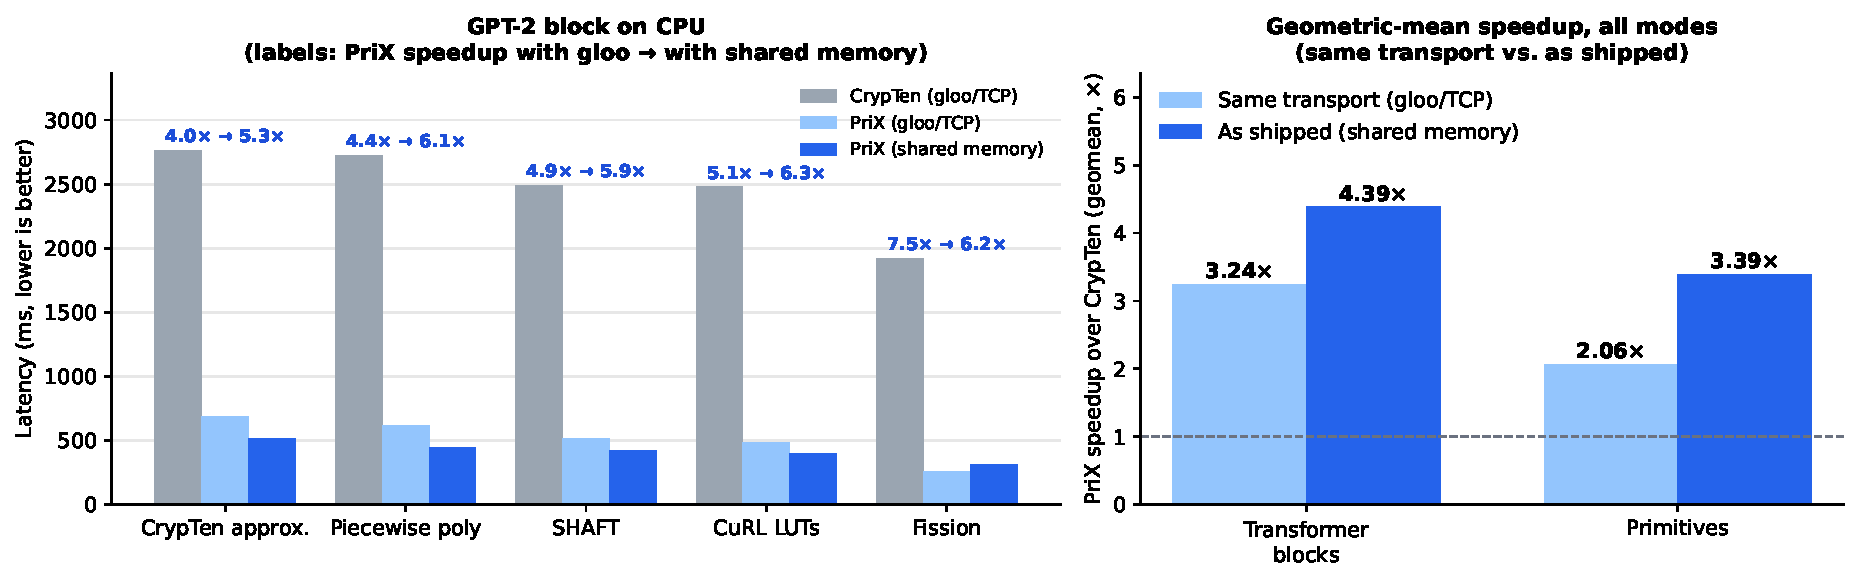
\includegraphics[width=\textwidth]{figures/transport_ablation.pdf}
\caption{Transport comparison on CPU. Left: GPT-2 block latency for CrypTen and for PriX over \texttt{gloo}, its own TCP transport (default), and shared memory; labels give PriX's speedup with its default transport. Right: geometric-mean speedup over all modes for each PriX transport.}
\label{fig:ablation}
\end{figure}

\begin{itemize}
    \item \textbf{Most of the speedup does not depend on the transport.} Even over CrypTen's own \texttt{gloo} transport, PriX is 3.14$\times$ faster than CrypTen on Transformer blocks on CPU (2.50--3.73$\times$ across modes) and 2.17$\times$ on GPU (1.94--2.47$\times$), and 1.92$\times$ (CPU) / 2.17$\times$ (GPU) faster on primitives.
    \item \textbf{CrypTen's \texttt{gloo} path is slower than a lean TCP transport.} PriX's own TCP transport is 1.32$\times$ faster than \texttt{gloo} on CPU blocks (1.51$\times$ on primitives) and 1.07$\times$ faster on GPU blocks (1.24$\times$ on primitives), so part of CrypTen's latency is its transport: \texttt{gloo} adds tensor conversions and collective-library overhead to every opening.
    \item \textbf{Shared memory adds little over TCP.} PriX over shared memory is only 4--5\% faster than over TCP on blocks (4.31$\times$ vs.\ 4.14$\times$ on CPU; 2.46$\times$ vs.\ 2.33$\times$ on GPU), and 22\% (CPU) / 6\% (GPU) faster on the small, round-bound primitives, where per-round latency dominates. For openings above 16\,MiB, TCP is faster, because the shared-memory transport falls back to pickled queues (46 vs.\ 162\,ms for a 19\,MB opening). We therefore made TCP the default; shared memory remains available as a single-host shortcut.
    \item \textbf{Fission mode depends least on the transport}, because it needs very few rounds between the MPC parties (about 14 per GPT-2 block, versus 98--176 in the other modes).
    \item \textbf{Communication is similar, but not identical.} In \texttt{crypten} mode, the two frameworks' round counts agree to within one round and their byte counts to within 5\% on every Transformer block (e.g.\ 176 rounds and 80.1 vs.\ 79.7\,MB for a GPT-2 block). Two PriX protocol changes account for most of the remaining differences:
    \begin{itemize}
        \item \emph{Smaller comparison openings.} In each carry-lookahead round, one masked vector $P_0$ is ANDed with both $S_1$ and $P_1$. CrypTen first copies $P_0$ to the shape of $[S_1, P_1]$ and therefore masks and opens it twice (its source marks this with a TODO); PriX uses a triple $(a, [b_1, b_2], [a \wedge b_1, a \wedge b_2])$ and opens $P_0 \oplus a$ once, as matrix Beaver triples do for a shared operand. The opened values are still uniformly masked by fresh triples, so security is unchanged. This cuts a comparison from 29 to 23 words per element (ReLU: 0.38 vs.\ 0.48\,MB), and \texttt{poly}-mode blocks send 5--16\% fewer bytes (GPT-2: 88.8 vs.\ 96.4\,MB).
        \item \emph{Batched range tests in SHAFT.} PriX obtains $[x < 0]$ and $[|x| < w]$ from one comparison over the stacked tensor $[x, x - w, -x - w]$, while the SHAFT reference runs two sequential comparisons. This saves 8 rounds per $\operatorname{GeLU}$/$\operatorname{SiLU}$ (11 vs.\ 19) and per SHAFT-mode block (GPT-2: 98 vs.\ 106), at the cost of about 4\% more bytes.
    \end{itemize}
    PriX takes more rounds in two places, both because it applies a configuration setting that the CrypTen code ignores. In \texttt{curl} mode, Curl truncates squares with the communication-free local shift even though the mode specifies $\mathsf{TruncPr}$ for products (its multiplications do use $\mathsf{TruncPr}$); PriX uses $\mathsf{TruncPr}$ for both, so its LayerNorm takes one extra round and each block two (GPT-2: 113 vs.\ 111). In \texttt{crypten} mode, CrypTen's sigmoid sets $\exp$ to 9 squarings in a configuration override that does not enclose the $\exp$ call, so it runs with the default 8; PriX applies the override, so its SiLU takes 25 rounds versus 24 and is about twice as accurate (Section~\ref{sec:accuracy}). Apart from \texttt{shaft} mode, PriX's speedups therefore do not come from fewer rounds.
\end{itemize}
We also recorded the time spent inside communication calls, but for PriX this does not separate cleanly from computation. JAX dispatches device work asynchronously, and the copy to the host at the start of each communication call waits for that work to finish, so compute time is attributed to communication. The transport swap above avoids this problem because it compares end-to-end latencies.

\subsection{Approximation Accuracy and Valid Input Ranges}
\label{sec:accuracy}
The latency results above say nothing about whether each mode computes the right function. Table~\ref{tab:accuracy} reports the error of each nonlinearity in PriX's default configuration of each mode, measured on CPU with two parties against exact float64 results (\texttt{benchmarks/accuracy\_sweep.py}). Each function is evaluated 10 times on a fixed grid of 241--257 points (softmax: $4 \times 32 \times 32$ logits drawn from $\mathcal{N}(0, 2^2)$; LayerNorm: $4 \times 32 \times 64$ inputs from $\mathcal{N}(0.5, 2^2)$), because probabilistic truncation and the masks make the error vary between runs.

\begin{table}[t]
\centering
\caption{\textbf{Approximation error by mode} (default configuration of each mode, 2 parties, 10 runs, CPU). Each cell is the median absolute error / the typical (median over runs) worst-case absolute error within one run. Bold marks a worst-case error above 0.1; $^\dagger$ marks functions for which at least one run had an error above 1.}
\label{tab:accuracy}
\vspace{2pt}
\footnotesize
\begin{tabular}{@{}lrrrrr@{}}
\toprule
\textbf{Function (inputs)} & \texttt{crypten} & \texttt{poly} & \texttt{shaft} & \texttt{curl} & \texttt{fission} \\
\midrule
$\exp$, $[-8, 0]$         & 4e-4 / 1e-3 & 2e-3 / 0.011 & 4e-4 / 1e-3 & 3e-4 / \textbf{0.12} & 4e-6 \\
$\exp$, $[-4, 2]$         & 1e-3 / 0.070 & 3e-3 / 0.011 & 1e-3 / 0.056 & 9e-3 / \textbf{7.4}$^\dagger$ & 5e-6 \\
$\log$, $[0.1, 50]$       & 0.020 / 0.033 & 0.020 / 0.032 & 0.020 / 0.033 & 1e-5 / \textbf{2.0}$^\dagger$ & 4e-6 \\
$1/x$, $[0.1, 50]$        & 9e-5 / 6e-4 & 9e-5 / 6e-4 & 9e-5 / 6e-4 & 7e-6 / \textbf{1.6e4}$^\dagger$ & 3e-6 \\
$1/\sqrt{x}$, $[0.05, 50]$ & 2e-5 / \textbf{0.24} & 2e-5 / \textbf{0.24} & 2e-5 / \textbf{0.24} & \textbf{0.13} / \textbf{193}$^\dagger$ & 4e-6 \\
Sigmoid, $[-8, 8]$        & 2e-4 / 2e-3 & 1e-3 / 9e-3 & 0.019 / \textbf{0.50} & 5e-5 / 4e-3 & 4e-6 \\
Tanh, $[-6, 6]$           & 1e-4 / 4e-3 & 1e-3 / 0.018 & 0.035 / 0.093 & 2e-5 / 9e-3 & 3e-6 \\
Erf, $[-4, 4]$            & \textbf{0.24} / \textbf{7.2e4}$^\dagger$ & 2e-3 / 0.015 & 0.027 / 0.071 & 5e-5 / 0.011 & 3e-6 \\
GeLU, $[-6, 6]$           & \textbf{0.92} / \textbf{1.4e6}$^\dagger$ & 4e-4 / 4e-3 & 4e-4 / 4e-3 & 3e-4 / \textbf{0.13} & 3e-6 \\
SiLU, $[-8, 8]$           & 6e-4 / 2e-3 & 5e-3 / 0.015 & 6e-4 / 5e-3 & 3e-3 / \textbf{0.32} & 4e-6 \\
Softmax                   & 1e-4 / 4e-3 & 6e-4 / 6e-3 & 3e-4 / 0.052 & 1e-4 / 0.015 & 4e-6 \\
LayerNorm                 & 9e-6 / 9e-5 & 9e-6 / 8e-5 & 1e-5 / 1e-4 & 1e-5 / 9e-5 & 4e-6 \\
\bottomrule
\end{tabular}
\end{table}

No mode is accurate everywhere, and inputs outside a mode's valid range are neither clamped nor flagged:
\begin{itemize}
    \item \textbf{\texttt{curl} (wavelet LUTs).} Curl's original defaults cover narrow ranges ($[0, 2)$ for $1/\sqrt{x}$ and $|x| < 4$ for GeLU, which caused LayerNorm to wrap whenever a row's variance was 2 or more and GeLU to wrap for $|x| \ge 4$) and suffer from an intermittent Softmax failure ($\approx -461$ on 3--4\% of calls in both PriX and the Curl reference). Tracing the wavelet tables explains the Softmax failure: Biorthogonal-2.2's decomposition filter has negative side lobes ($-1/8$), so the $1/x$ pole at $x = 2^{-16}$ gives bin $k = 1$ of the reciprocal table a large negative knot ($\approx -4968$). With Curl's $2^7$-bin reciprocal table on $[0, 64)$, bin $k = 1$ spans $[0.5, 1.0)$, while Curl's $2^5$-bin negative-exponential table on $[0, 64)$ evaluates $\widehat{\exp}(0) = 0.924 < 1$. Whenever a Softmax row has one dominant logit, the sum of exponentials falls in $[0.924, 1.0)$ and lands in bin $k = 1$ whenever $\mathsf{TruncPr}$ rounds down. PriX therefore sets \texttt{inv\_sqrt.lut\_max\_bits} $= 4$ ($[0, 16)$), \texttt{gelu.lut\_max\_bits} $= 3$ ($[-8, 8]$), \texttt{exp.lut\_max\_bits} $= 4$ ($\widehat{\exp}(0) = 0.992$), and \texttt{reciprocal.bior\_size\_bits} $= 8$ (moving $[0.75, 1.0)$ to bin $k = 3$), which fixes LayerNorm, GeLU on $[-6, 6]$, and Softmax without changing the table sizes or the communication volume (the latency benchmarks above use these defaults in both frameworks). Even with these defaults, $1/\sqrt{x}$ wraps for $x \ge 16$, $\exp$ assumes non-positive inputs (\texttt{all\_neg = True}), and $1/x$, $1/\sqrt{x}$, and $\log$ remain inaccurate in their first two bins near 0 because of the Biorthogonal-2.2 boundary sidelobe.
    \item \textbf{\texttt{crypten}.} Erf and GeLU use an 8-term Taylor series that is accurate to $3 \times 10^{-4}$ on $|x| \le 1.75$ (GeLU: $10^{-4}$ on $|x| \le 2.0$) but diverges for $|x| \gtrsim 2.5$, as in CrypTen. The Newton--Raphson $1/\sqrt{x}$ loses accuracy near the bottom of its range.
    \item \textbf{\texttt{shaft}.} The Fourier series are periodic, so Sigmoid and Tanh oscillate near the edge of the period ($|x| \approx 8$ by default).
    \item \textbf{\texttt{poly}} stays within about 0.02 on its fitted intervals, and \textbf{\texttt{fission}} is exact to float32 precision (its column shows the median error only).
\end{itemize}
\paragraph{Comparison with the CrypTen/Curl reference.} On identical inputs (10 runs each), PriX is more accurate than the reference implementation on three functions, because of three bugs in the reference code rather than any protocol difference. (1)~CrypTen's \texttt{var()} inverts its \texttt{unbiased} flag and divides by $n - 1$ when asked for the biased variance, so every non-\texttt{fission} LayerNorm output is scaled by $\sqrt{(n-1)/n}$ ($0.9922$ for $n = 64$; a least-squares fit of Curl's outputs gives $0.9921$). Curl's \texttt{curl}-mode LayerNorm has a median error of $5.4 \times 10^{-3}$ versus $1.0 \times 10^{-5}$ for PriX; the bias shrinks with width (about $0.07\%$ at $d = 768$). (2)~The ineffective $\exp$ override described in Section~\ref{sec:ablation} roughly doubles the error of CrypTen's \texttt{crypten}-mode SiLU (median $1.1 \times 10^{-3}$ versus $5.6 \times 10^{-4}$). (3)~CrypTen's integer \texttt{pow(p)} computes $(x^3)^{(p-1)/2} = x^{3(p-1)/2}$ instead of $(x^2)^{(p-1)/2} \cdot x = x^p$ for odd $p \ge 5$, which replaces odd powers $x^5, x^9, x^{13}, x^{17}$ in its Taylor \texttt{erf} with even powers $x^6, x^{12}, x^{18}, x^{24}$ (raising its \texttt{erf} error on $[-1.5, 1.5]$ from $3 \times 10^{-4}$ to $3.3$ and its median error on $[-4, 4]$ from $0.24$ to $2.5 \times 10^3$). None of these bugs changes the number of multiplications or the cost of the computation, so the latency comparison is unaffected.
While preparing this evaluation, we found and fixed a bug in PriX's \texttt{fission} mode: when the right operand of a multiplication still carried a deferred truncation, the product was labelled with the wrong fixed-point scale, which made attention scores about $2^{16}$ times too small and attention nearly uniform. The fix changes only the scale label, not the protocol steps that run, so it does not affect the latencies above, which were measured before it. The reference implementations of Curl and Fission in the CrypTen baseline do not have this bug. We have not measured end-to-end model accuracy.

%======================================================================
\section{Protocol Case Studies: Function Secret Sharing, Wavelets, and Truncation Trade-offs}
\label{sec:fss_wave_discussion}
%======================================================================

Because PriX executes distinct cryptographic paradigms inside the same compiled JAX/XLA runtime, transport, and fixed-point representation, it enables controlled cross-paradigm comparisons that are otherwise confounded by differences in implementation language, hardware backend, or ring bitwidth. In this section, we use PriX to investigate three questions raised by recent literature:
(1)~How do Function Secret Sharing (FSS) protocols---\textbf{SIGMA}~\cite{gupta2024sigma} and \textbf{Wave}~\cite{reis2025wave}---compare against \textbf{SHAFT}~\cite{kei2025shaft} and \textbf{Curl}~\cite{santos2024curl} when evaluated on an equal footing?
(2)~How does Wave's deterministic DPF/DCF LUT truncation (\texttt{lut\_indexing="wave"}) compare against its probabilistic local-shift variant (\texttt{lut\_indexing="wave\_prob"})?
(3)~Why does CrypTen's 0-round local product truncation (\texttt{truncation="crypten"}) exhibit near-zero error on standard single-block benchmarks despite being known to fail catastrophically in general?

\subsection{Function Secret Sharing in PriX: SIGMA and Wave}
\label{sec:fss_impl}

In addition to secret-shared carry-lookahead circuits and one-hot LUT correlations, PriX implements 2-party Function Secret Sharing~\cite{boyle2015function,boyle2016function} in \texttt{prix/fss.py}, compiling PRG tree traversal (\texttt{jax.lax.fori\_loop}) and Grotto prefix-parity evaluation~\cite{storrier2023grotto} into fused XLA executables:
\begin{itemize}
    \item \textbf{Faithful SIGMA Protocols (\texttt{mode="sigma"}, \texttt{lut\_indexing="sigma"})}~\cite{gupta2024sigma}: Rather than running 6 interactive rounds of Kogge--Stone AND gates for $\shareA{x} < 0$, parties mask the input $\hat{x} = x + r$ in 1 online round ($8\,\text{B}$) and locally evaluate a Grotto Distributed Point Function (DPF) prefix-parity tree to obtain XOR shares of the comparison bit $\shareB{x < 0}$, followed by 1 round of binary-to-arithmetic conversion or multiplexed selection (2 online rounds total, versus 8 rounds in SPK). For nonlinearities, \texttt{mode="sigma"} implements SIGMA's exact two-phase protocols from~\cite{gupta2024sigma} (Figures~7--9, Table~2):
    \begin{enumerate}
        \item \emph{Symmetry, clipping, and Truncate-Reduce ($\Pi^{\text{TR}}_{n,f}$) before LUT lookup:} Because raw 0th-order lookup tables scale exponentially with bitwidth, SIGMA first executes online DPF comparisons and $\Pi^{\text{Select}}$ multiplexers to fold negative inputs and clamp the domain before calling a small table, followed by a 1-round faithful Truncate-Reduce ($\Pi^{\text{TR}}_{n,f}$, Theorem~4) opening to drop low fractional bits before the 2-round DPF-LUT evaluation ($3\,\text{rounds}, 32\,\text{B}$/element per LUT). Specifically, $\operatorname{GeLU}(x) = \operatorname{ReLU}(x) - \operatorname{LUT}_{256}(\operatorname{Clip}(|x|, 0, 4))$ and $\operatorname{SiLU}(x) = \operatorname{ReLU}(x) - \operatorname{LUT}_{1024}(\operatorname{Clip}(|x|, 0, 8))$ require \textbf{6 online rounds and $56.3\,\text{B}$/element} (matching SIGMA Table~2's $58\,\text{B}$); $\exp(-x)$ (Figure~8) clips to $[0, 16)$, runs $\Pi^{\text{TR}}$, evaluates two $2^8$-entry tables $\exp(-z_{\text{high}})\cdot\exp(-z_{\text{low}})$ via a Beaver multiplication, and muxes clipped inputs (\textbf{12 rounds, $120.1\,\text{B}$/element}); and $1/\sqrt{x}$ (Figure~9) uses tailored range checks plus aLUT + Newton--Raphson refinement (\textbf{10 rounds, $104.1\,\text{B}$/element}, matching SIGMA Table~2's $106\,\text{B}$).
    \end{enumerate}
    \item \textbf{Deterministic Wave (\texttt{mode="wave"}, \texttt{lut\_indexing="wave"})}~\cite{reis2025wave}: Wave bridges FSS and wavelet-compressed lookup tables in two ways: (i)~because wavelet basis functions are compactly supported on $[-2^{\max}, 2^{\max})$, Wave encodes the entire activation (including sign and tail) directly into a single wavelet coefficient table, eliminating SIGMA's pre-LUT sign/clip comparisons, multiplexers, and $\Pi^{\text{TR}}$ round; and (ii)~it replaces 0th-order step tables with 1st-order piecewise-linear Biorthogonal $\text{bior}(5,3)$ (LeGall) splines (and Haar $\text{bior}(1,1)$ where appropriate), shrinking table sizes by $16\times$--$64\times$. For a table of $2^J$ coarse intervals with step size $2^{\mathfrak{j}}$, parties open $\hat{x} = x + r \bmod 2^{J+\mathfrak{j}}$ in Round~1 ($8\,\text{B}$) and locally evaluate:
    \begin{enumerate}
        \item a \emph{$(J+\mathfrak{j})$-level Grotto DPF} (\texttt{grotto\_segment\_parities\_jit}) that outputs exact XOR shares of the one-hot indicator $\shareB{\mathbf{e}_k} \in \{0,1\}^{2^J}$ for the coarse bin $k = \lfloor x / 2^{\mathfrak{j}} \rfloor$ \emph{without} a separate $\Pi^{\text{TR}}$ round and without off-by-1 probabilistic truncation error at interval boundaries; and
        \item a \emph{$\mathfrak{j}$-level arithmetic Distributed Comparison Function (DCF)} (\texttt{dcf\_eval\_arith\_jit}) that computes the exact low-bit borrow $\shareA{\mathbb{I}[\hat{x}_{\text{low}} < r_{\text{low}}]}$ in 0 extra rounds, yielding exact additive shares of the intra-bin offset $\shareA{x_{\text{low}}} = \hat{x}_{\text{low}} - \shareA{r_{\text{low}}} - 2^{\mathfrak{j}}\shareA{\mathbb{I}[\hat{x}_{\text{low}} < r_{\text{low}}]}$.
    \end{enumerate}
    In Round~2, Wave's $\Pi^{\text{LUT-bior(5,3)}}$ protocol (\texttt{wave\_bior\_lut}) uses a generalized Beaver 8-tuple $(\tau_0, \tau_1, \theta, \alpha_0, \alpha_1, \beta_0, \beta_1, \gamma)$ to simultaneously convert the XOR-shared slope and intercept $(v_0, v_1)$ into arithmetic shares over $\Zring$ and multiply $v_0 \cdot \shareA{x_{\text{low}}}$ in a single $32\,\text{B}$ opening. This evaluates a piecewise-linear wavelet LUT in \textbf{2 online rounds and $40\,\text{B}$/element}---cutting SIGMA's 6--12 rounds to 2, halving Curl's 4 rounds, and eliminating boundary jump errors.
    \item \textbf{Probabilistic Wave (\texttt{lut\_indexing="wave\_prob"})}: Following Wave~\S5.3, PriX also supports a probabilistic truncation variant (\texttt{\_wave\_bior\_prob\_r1\_jit}) that locally splits $\shareA{x}$ in 0 rounds via
    \begin{equation}
        x_{\text{high}, b} = (x_b \gg \mathfrak{j}) + \mathbb{I}[b = 0], \qquad
        x_{\text{lsb}, b} = \big(x_b \mathbin{\&} (2^{\mathfrak{j}} - 1)\big) - \mathbb{I}[b = 0]\cdot 2^{\mathfrak{j}},
        \label{eq:wave_prob_split}
    \end{equation}
    which preserves the exact identity $x_{\text{high}} \cdot 2^{\mathfrak{j}} + x_{\text{lsb}} = x$ while guaranteeing $x_{\text{high}} \in \{k, k+1\}$ (preventing bin $0$ from wrapping to $2^J - 1$). Because $x_{\text{high}}$ is already truncated to $J$ bits, parties evaluate only a $J$-level DPF with no $\mathfrak{j}$-level DPF tail and no arithmetic DCF.
\end{itemize}

\subsection{Re-evaluating SHAFT vs.\ SIGMA, Wave, and Curl under a Unified Runtime}
\label{sec:shaft_vs_sigma_wave}

SHAFT~\cite{kei2025shaft} (Table~VII) reported $3.7\times$--$6.4\times$ lower $\operatorname{GeLU}$ latency and $1.4\times$--$2.5\times$ lower end-to-end Transformer latency than SIGMA~\cite{gupta2024sigma}, attributing these gains to replacing lookup tables with 1-round Fourier series and ODE $\operatorname{Softmax}$. However, that comparison benchmarked SHAFT's Python/CrypTen code at $f=16$ against SIGMA's standalone C++/CUDA binary over 37--50-bit rings. Tables~\ref{tab:wave_primitives} and~\ref{tab:wave_e2e} compare \textbf{Wave} (\texttt{mode="wave"}), \textbf{SIGMA} (\texttt{mode="sigma"}), \textbf{Curl} (\texttt{mode="curl"}), and \textbf{SHAFT} (\texttt{mode="shaft"}) inside PriX on CPU across primitive nonlinearities, \texttt{BERT-base} sublayers ($L=128$), and full 12- and 24-layer Transformer models.

\begin{table}[t]
\centering
\caption{\textbf{Cross-paradigm comparison of Wave, SIGMA, Curl, and SHAFT on primitive nonlinearities ($N=1000$ elements)} in PriX (2 parties, CPU, $f=16$). We report online communication rounds, per-party online communication (bytes/element), local CPU execution time (ms), and mean absolute error (MAE) against float64.}
\label{tab:wave_primitives}
\vspace{2pt}
\footnotesize
\resizebox{\textwidth}{!}{%
\begin{tabular}{@{}llcccc@{}}
\toprule
\textbf{Primitive (Range)} & \textbf{Metric} & \textbf{Wave (\texttt{mode="wave"})} & \textbf{SIGMA (\texttt{mode="sigma"})} & \textbf{Curl (\texttt{mode="curl"})} & \textbf{SHAFT (\texttt{mode="shaft"})} \\
\midrule
\multirow{2}{*}{$\operatorname{GeLU}$ ($[-3.8, 3.8]$)}
 & Rounds / Comm (1P) & \textbf{2 rds} / $\mathbf{40.0\,\text{B}}$ & 6 rds / $56.3\,\text{B}$ & 4 rds / $\mathbf{40.0\,\text{B}}$ & 11 rds / $544.0\,\text{B}$ \\
 & Time / MAE & $\mathbf{10.5\,\text{ms}}$ / $1.75\times 10^{-3}$ & $28.8\,\text{ms}$ / $\mathbf{3.49\times 10^{-4}}$ & $15.1\,\text{ms}$ / $9.07\times 10^{-3}$ & $15.5\,\text{ms}$ / $9.41\times 10^{-4}$ \\
\midrule
\multirow{2}{*}{$\operatorname{SiLU}$ ($[-7.5, 7.5]$)}
 & Rounds / Comm (1P) & \textbf{2 rds} / $\mathbf{40.0\,\text{B}}$ & 6 rds / $56.3\,\text{B}$ & 4 rds / $\mathbf{40.0\,\text{B}}$ & 11 rds / $544.0\,\text{B}$ \\
 & Time / MAE & $7.9\,\text{ms}$ / $3.47\times 10^{-3}$ & $32.4\,\text{ms}$ / $\mathbf{4.96\times 10^{-4}}$ & $\mathbf{7.2\,\text{ms}}$ / $1.69\times 10^{-2}$ & $23.1\,\text{ms}$ / $8.55\times 10^{-4}$ \\
\midrule
\multirow{2}{*}{$\operatorname{Sigmoid}$ ($[-7.5, 7.5]$)}
 & Rounds / Comm (1P) & 6 rds / $80.3\,\text{B}$ & 7 rds / $72.3\,\text{B}$ & 15 rds / $592.0\,\text{B}$ & \textbf{1 rd} / $\mathbf{8.0\,\text{B}}$ \\
 & Time / MAE & $36.8\,\text{ms}$ / $\mathbf{7.24\times 10^{-5}}$ & $26.5\,\text{ms}$ / $4.16\times 10^{-3}$ & $21.7\,\text{ms}$ / $3.70\times 10^{-4}$ & $\mathbf{3.2\,\text{ms}}$ / $2.24\times 10^{-2}$ \\
\midrule
\multirow{2}{*}{$\operatorname{Tanh}$ ($[-4.5, 4.5]$)}
 & Rounds / Comm (1P) & 6 rds / $80.3\,\text{B}$ & 7 rds / $72.3\,\text{B}$ & 15 rds / $592.0\,\text{B}$ & \textbf{1 rd} / $\mathbf{8.0\,\text{B}}$ \\
 & Time / MAE & $32.0\,\text{ms}$ / $\mathbf{1.17\times 10^{-4}}$ & $21.3\,\text{ms}$ / $6.93\times 10^{-3}$ & $23.2\,\text{ms}$ / $5.24\times 10^{-4}$ & $\mathbf{1.8\,\text{ms}}$ / $3.03\times 10^{-2}$ \\
\midrule
\multirow{2}{*}{$\operatorname{Erf}$ ($[-3.5, 3.5]$)}
 & Rounds / Comm (1P) & 9 rds / $104.3\,\text{B}$ & 10 rds / $96.3\,\text{B}$ & 23 rds / $424.0\,\text{B}$ & \textbf{1 rd} / $\mathbf{8.0\,\text{B}}$ \\
 & Time / MAE & $37.6\,\text{ms}$ / $\mathbf{1.68\times 10^{-4}}$ & $34.3\,\text{ms}$ / $8.93\times 10^{-3}$ & $29.0\,\text{ms}$ / $8.29\times 10^{-4}$ & $\mathbf{2.8\,\text{ms}}$ / $2.37\times 10^{-2}$ \\
\midrule
\multirow{2}{*}{$\operatorname{nexp}$ ($\exp(x), [-15, 0)$)}
 & Rounds / Comm (1P) & \textbf{5 rds} / $64.1\,\text{B}$ & 12 rds / $120.1\,\text{B}$ & 13 rds / $224.0\,\text{B}$ & 8 rds / $\mathbf{64.0\,\text{B}}$ \\
 & Time / MAE & $\mathbf{12.3\,\text{ms}}$ / $6.04\times 10^{-4}$ & $38.7\,\text{ms}$ / $\mathbf{1.13\times 10^{-5}}$ & $13.0\,\text{ms}$ / $2.24\times 10^{-3}$ & $12.5\,\text{ms}$ / $3.09\times 10^{-4}$ \\
\midrule
\multirow{2}{*}{$1/x$ ($[1.0, 30.0]$)}
 & Rounds / Comm (1P) & \textbf{2 rds} / $40.0\,\text{B}$ & 3 rds / $\mathbf{32.0\,\text{B}}$ & 4 rds / $40.0\,\text{B}$ & 28 rds / $304.0\,\text{B}$ \\
 & Time / MAE & $31.6\,\text{ms}$ / $8.51\times 10^{-5}$ & $20.7\,\text{ms}$ / $5.36\times 10^{-4}$ & $\mathbf{10.0\,\text{ms}}$ / $3.42\times 10^{-4}$ & $56.2\,\text{ms}$ / $\mathbf{8.08\times 10^{-5}}$ \\
\midrule
\multirow{2}{*}{$1/\sqrt{x}$ ($[0.1, 15.0]$)}
 & Rounds / Comm (1P) & \textbf{2 rds} / $\mathbf{40.0\,\text{B}}$ & 10 rds / $104.1\,\text{B}$ & 4 rds / $\mathbf{40.0\,\text{B}}$ & 17 rds / $184.0\,\text{B}$ \\
 & Time / MAE & $97.1\,\text{ms}$ / $\mathbf{2.61\times 10^{-5}}$ & $45.8\,\text{ms}$ / $2.25\times 10^{-4}$ & $\mathbf{15.6\,\text{ms}}$ / $1.03\times 10^{-4}$ & $22.0\,\text{ms}$ / $4.65\times 10^{-4}$ \\
\bottomrule
\end{tabular}%
}
\end{table}

\begin{table}[t]
\centering
\caption{\textbf{Sublayer ($L=128$) and end-to-end Transformer comparison of Wave, SIGMA, Curl, and SHAFT} in PriX (2 parties, CPU, $f=16$). Total 2P Comm reports combined online traffic sent by both parties.}
\label{tab:wave_e2e}
\vspace{2pt}
\footnotesize
\resizebox{\textwidth}{!}{%
\begin{tabular}{@{}llcccc@{}}
\toprule
\textbf{Benchmark} & \textbf{Metric} & \textbf{Wave (\texttt{mode="wave"})} & \textbf{SIGMA (\texttt{mode="sigma"})} & \textbf{Curl (\texttt{mode="curl"})} & \textbf{SHAFT (\texttt{mode="shaft"})} \\
\midrule
\multirow{3}{*}{$\operatorname{GeLU}$ $(1, 128, 3072)$}
 & Rounds / 2P Comm & \textbf{2 rds} / $\mathbf{31.46\,\text{MB}}$ & 6 rds / $44.24\,\text{MB}$ & 4 rds / $\mathbf{31.46\,\text{MB}}$ & 11 rds / $427.82\,\text{MB}$ \\
 & Local Time (s) & $1.66\,\text{s}$ & $2.60\,\text{s}$ & $\mathbf{0.13\,\text{s}}$ & $0.52\,\text{s}$ \\
 & MAE / Max Error & $0.00190$ / $0.0158$ & $\mathbf{0.00038}$ / $\mathbf{0.0039}$ & $0.00979$ / $0.2096$ & $0.00098$ / $0.0045$ \\
\midrule
\multirow{3}{*}{$\operatorname{Softmax}$ $(1, 12, 128, 128)$}
 & Rounds / 2P Comm & \textbf{23 rds} / $\mathbf{34.82\,\text{MB}}$ & 31 rds / $56.82\,\text{MB}$ & 98 rds / $311.87\,\text{MB}$ & 41 rds / $346.03\,\text{MB}$ \\
 & Local Time (s) & $1.77\,\text{s}$ & $2.16\,\text{s}$ & $0.64\,\text{s}$ & $\mathbf{0.63\,\text{s}}$ \\
 & MAE / Max Error & $6.78\times 10^{-5}$ / $0.00093$ & $\mathbf{8.68\times 10^{-6}}$ / $\mathbf{0.00012}$ & $2.81\times 10^{-4}$ / $0.00715$ & $2.41\times 10^{-4}$ / $0.00522$ \\
\midrule
\multirow{3}{*}{$\operatorname{LayerNorm}$ $(1, 128, 768)$}
 & Rounds / 2P Comm & \textbf{6 rds} / $6.30\,\text{MB}$ & 14 rds / $6.32\,\text{MB}$ & 8 rds / $6.30\,\text{MB}$ & 19 rds / $\mathbf{3.19\,\text{MB}}$ \\
 & Local Time (s) & $0.226\,\text{s}$ & $0.065\,\text{s}$ & $0.056\,\text{s}$ & $\mathbf{0.053\,\text{s}}$ \\
 & MAE / Max Error & $2.98\times 10^{-5}$ / $\mathbf{0.00020}$ & $1.13\times 10^{-3}$ / $0.00961$ & $\mathbf{2.80\times 10^{-5}}$ / $0.00041$ & $8.48\times 10^{-4}$ / $0.00551$ \\
\midrule
\multirow{4}{*}{\texttt{BERT-base} (12L, $L=128$)}
 & Rounds / Block (Total) & \textbf{58} (\textbf{696}) & 86 (1,032) & 139 (1,668) & 100 (1,200) \\
 & Total 2P Comm (GB) & $\mathbf{1.551\,\text{GB}}$ & $1.968\,\text{GB}$ & $6.234\,\text{GB}$ & $11.024\,\text{GB}$ \\
 & Local Runtime (12L) & $50.56\,\text{s}$ & $65.90\,\text{s}$ & $\mathbf{17.95\,\text{s}}$ & $20.50\,\text{s}$ \\
 & Block MAE & $0.0028$ & $0.0017$ & $0.0191$ & $\mathbf{0.0015}$ \\
\midrule
\multirow{4}{*}{\texttt{BERT-large} (24L, $L=128$)}
 & Rounds / Block (Total) & \textbf{58} (\textbf{1,392}) & 86 (2,064) & 139 (3,336) & 100 (2,400) \\
 & Total 2P Comm (GB) & $\mathbf{4.135\,\text{GB}}$ & $5.248\,\text{GB}$ & $17.833\,\text{GB}$ & $30.605\,\text{GB}$ \\
 & Local Runtime (24L) & $140.01\,\text{s}$ & $189.40\,\text{s}$ & $\mathbf{55.29\,\text{s}}$ & $61.77\,\text{s}$ \\
 & Block MAE & $0.0028$ & $0.0016$ & $0.0192$ & $\mathbf{0.0015}$ \\
\midrule
\multirow{4}{*}{\texttt{GPT-2} (12L, $L=64$)}
 & Rounds / Block (Total) & \textbf{56} (\textbf{672}) & 84 (1,008) & 138 (1,656) & 100 (1,200) \\
 & Total 2P Comm (GB) & $\mathbf{0.643\,\text{GB}}$ & $0.786\,\text{GB}$ & $2.782\,\text{GB}$ & $5.144\,\text{GB}$ \\
 & Local Runtime (12L) & $24.16\,\text{s}$ & $27.65\,\text{s}$ & $12.85\,\text{s}$ & $\mathbf{12.28\,\text{s}}$ \\
 & Block MAE & $0.0028$ & $\mathbf{0.0015}$ & $0.0194$ & $\mathbf{0.0015}$ \\
\bottomrule
\end{tabular}%
}
\end{table}

Three findings emerge from Tables~\ref{tab:wave_primitives} and~\ref{tab:wave_e2e}:
\begin{enumerate}
    \item \textbf{Disentangling SHAFT vs.\ SIGMA:} First, our \texttt{mode="sigma"} implementation reproduces SIGMA's reported per-party communication~\cite{gupta2024sigma} (Tables~2, 3, 5, and~8): $56.3\,\text{B}$/element on $\operatorname{GeLU}/\operatorname{SiLU}$ (vs.\ $58\,\text{B}$ in SIGMA), $32.0\,\text{B}$ on $1/x$ (vs.\ $36\,\text{B}$), $104.1\,\text{B}$ on $1/\sqrt{x}$ (vs.\ $106\,\text{B}$), $0.265\,\text{GB}$ per party across 12 \texttt{BERT-base} $\operatorname{GeLU}$ layers (vs.\ $0.26\,\text{GB}$ in SIGMA Table~3), $0.341\,\text{GB}$ across 12 $\operatorname{Softmax}$ layers (vs.\ $0.37\,\text{GB}$), and end-to-end 1-party model communication matching within $0.6\%$ ($\mathbf{0.984\,\text{GB}}$ vs.\ $\mathbf{0.99\,\text{GB}}$ on \texttt{BERT-base}; $\mathbf{2.624\,\text{GB}}$ vs.\ $\mathbf{2.64\,\text{GB}}$ on \texttt{BERT-large}; $\mathbf{0.393\,\text{GB}}$ vs.\ $\mathbf{0.37\,\text{GB}}$ on \texttt{GPT-2} at $L=64$). Comparing SHAFT against SIGMA on an equal footing reveals why their relative performance depends on the network regime: SHAFT's Fourier series requires 1 online round only when the input is guaranteed to stay within one half-period ($\operatorname{Sigmoid}$, $\operatorname{Tanh}$, $\operatorname{Erf}$). For unbounded activations ($\operatorname{GeLU}$ and $\operatorname{SiLU}$), SHAFT must first evaluate secure range-clipping comparisons ($[x < 0]$ and $[|x| < w]$), requiring \textbf{11 online rounds and $544\,\text{B}$/element} ($427.8\,\text{MB}$ on \texttt{BERT-base} $\operatorname{GeLU}$) compared with \textbf{6 rounds and $56.3\,\text{B}$/element} ($44.2\,\text{MB}$) for SIGMA and \textbf{2 rounds and $40.0\,\text{B}$/element} ($31.5\,\text{MB}$) for Wave. Across a 12-layer \texttt{BERT-base} ($L=128$), SHAFT requires \textbf{1,200 online rounds and $11.02\,\text{GB}$}, whereas SIGMA requires \textbf{1,032 rounds and $1.97\,\text{GB}$} ($5.6\times$ less communication) and Wave requires \textbf{696 rounds and $1.55\,\text{GB}$} ($1.72\times$ fewer rounds and $7.1\times$ less communication). Why is SHAFT faster than SIGMA in local CPU runtime inside JAX ($20.5\,\text{s}$ vs.\ $65.9\,\text{s}$)? Because XLA does not expose x86 hardware \texttt{AES-NI} intrinsics (\texttt{\_mm\_aesenc\_si128}) that C++ FSS engines use to evaluate 128-bit DPF nodes in a single hardware instruction; instead, JAX evaluates our 64-bit counter-mode PRG over 256- to 1024-leaf DPF trees per element ($2.60\,\text{s}$ on $\operatorname{GeLU}$, $24.3\,\text{ms}$ on $\operatorname{SiLU}$), whereas SHAFT evaluates a dense linear combination after its comparison rounds ($0.52\,\text{s}$). Over any wide-area network ($100\,\text{Mbps}$--$1\,\text{Gbps}$ bandwidth, $10$--$40\,\text{ms}$ RTT), SHAFT's $9.0$--$9.5\,\text{GB}$ of extra traffic adds $75$--$750+\,\text{s}$ of network transfer time, reversing its local-CPU advantage.
    \item \textbf{Wave vs.\ SIGMA (why Wave's wavelet representation improves rounds, communication, and compute simultaneously):} Replacing SIGMA's multi-phase 0th-order LUT protocols with Wave's 2-round $\text{bior}(5,3)$ wavelet LUTs wins on all three axes:
    \begin{itemize}
        \item \emph{$1.48\times$--$5\times$ fewer rounds:} Because wavelet basis functions are compactly supported, Wave encodes the full activation domain directly into a single wavelet LUT and folds exact bin truncation into the $(J+\mathfrak{j})$-level Grotto DPF + $\mathfrak{j}$-level arithmetic DCF. This eliminates SIGMA's pre-LUT sign/clip comparisons, multiplexers, and $\Pi^{\text{TR}}$ round---cutting $\operatorname{GeLU}/\operatorname{SiLU}$ from $6 \to 2$ rounds, $\operatorname{nexp}$ from $12 \to 5$ rounds, $1/\sqrt{x}$ from $10 \to 2$ rounds, $\operatorname{Softmax}$ from $31 \to 23$ rounds, $\operatorname{LayerNorm}$ from $14 \to 6$ rounds, and a full Transformer block from \textbf{$86 \to 58$ rounds ($1,032 \to 696$ on \texttt{BERT-base})}.
        \item \emph{$21\%$--$62\%$ lower communication:} Wave cuts per-element traffic from $56.3 \to 40.0\,\text{B}$ on $\operatorname{GeLU}/\operatorname{SiLU}$ ($-29\%$), $120.1 \to 64.1\,\text{B}$ on $\operatorname{nexp}$ ($-47\%$), $104.1 \to 40.0\,\text{B}$ on $1/\sqrt{x}$ ($-62\%$), $56.8 \to 34.8\,\text{MB}$ on $\operatorname{Softmax}$ ($-39\%$), and \textbf{$1.968 \to 1.551\,\text{GB}$ on 12-layer \texttt{BERT-base} ($-21\%$)} ($5.248 \to 4.135\,\text{GB}$ on \texttt{BERT-large}).
        \item \emph{$1.2\times$--$3.5\times$ faster local CPU compute (2-round Wave; $2.9\times$--$4\times$ with SIGMA-TR indexing, Section~\ref{sec:keysize}):} Because 1st-order piecewise-linear $\text{bior}(5,3)$ splines represent smooth curves with \textbf{$16\times$--$64\times$ fewer LUT intervals} than SIGMA's 0th-order step tables ($2^4 = 16$ vs.\ $2^8 = 256$ knots on $\operatorname{GeLU}$, $2^4 = 16$ vs.\ $2^{10} = 1024$ on $\operatorname{SiLU}$, and one $2^5 = 32$ table vs.\ two $2^8 = 256$ tables on $\operatorname{nexp}$), Wave's Grotto DPF prefix tree evaluates $16\times$--$64\times$ fewer leaves per element---accelerating $\operatorname{GeLU}$ by \textbf{$1.6\times$} ($1.66\,\text{s}$ vs.\ $2.60\,\text{s}$), $\operatorname{SiLU}$ by \textbf{$3.5\times$} ($6.9\,\text{ms}$ vs.\ $24.3\,\text{ms}$), $\operatorname{Softmax}$ by \textbf{$1.2\times$} ($1.77\,\text{s}$ vs.\ $2.16\,\text{s}$), and end-to-end \texttt{BERT-base} / \texttt{BERT-large} by \textbf{$1.3\times$--$1.4\times$} ($50.6\,\text{s}$ vs.\ $65.9\,\text{s}$; $140.0\,\text{s}$ vs.\ $189.4\,\text{s}$).
    \end{itemize}
    \item \textbf{Wave vs.\ Curl:} Compared with Curl (\texttt{mode="curl"}), Wave reduces Transformer rounds by \textbf{$2.4\times$} ($58$ vs.\ $139$ rounds/block; $23$ vs.\ $98$ on $\operatorname{Softmax}$) and total online communication by \textbf{$4.0\times$--$4.3\times$} ($1.55\,\text{GB}$ vs.\ $6.23\,\text{GB}$ on \texttt{BERT-base}), while improving accuracy on every operation ($\operatorname{GeLU}$ max error drops $13\times$ from $0.2096$ to $0.0158$; \texttt{GPT-2} block MAE drops $6.8\times$ from $0.0190$ to $0.0028$) because deterministic DPF/DCF truncation eliminates off-by-1 knot boundary jumps.
\end{enumerate}

\subsection{Preprocessing Key Size, Wave with SIGMA's Truncate-Reduce, and What a Simulated Dealer Hides}
\label{sec:keysize}

\paragraph{Methodology caveat.} All latencies in this section are \emph{online-phase} numbers obtained with PriX's simulated dealer (\texttt{provider=TFP}): both parties expand the same PRG seeds, so the DPF/DCF correction words, Beaver tuples, and masks are derived locally and \textbf{no key material is ever transmitted}. This is the same convention as CrypTen's \texttt{TrustedFirstParty} and as the online columns of SIGMA~\cite{gupta2024sigma} and Wave~\cite{reis2025wave}, but it is \emph{not} a secure deployment (each party could recover the other's key), and it hides two costs that a real dealer incurs: (i)~the key must be generated by a third party or a 2PC key-generation protocol, and (ii)~the correction words---which depend on the secret offset $\alpha$ and on both parties' seeds---cannot be compressed to a seed and must be sent to each party. Note also that PriX runs the dealer's $\mathsf{Gen}$ \emph{inline} on the online path, so its compute is, if anything, over-counted. To make the hidden cost visible, PriX's providers now account the bytes of non-seed-derivable key material one party would receive (\texttt{prix.provider.get\_preproc\_stats}): one correction word per DPF level ($64$~bits for PriX's 62-bit seeds, re-counted at $\lambda=128$ as $16\,\text{B}$/level for a like-for-like comparison with SIGMA/Orca), seed and value correction words for arithmetic DCFs, and $64$~bits ($1$~bit) per shared ring (binary) element. As a sanity check, this accounting reproduces SIGMA Table~2's published key sizes: $1{,}488\,\text{B}$ vs.\ $1.43\,\text{KB}$ on $\operatorname{GeLU}$, $1{,}496\,\text{B}$ vs.\ $1.46\,\text{KB}$ on $\operatorname{SiLU}$, and $1{,}888\,\text{B}$ vs.\ $1.93\,\text{KB}$ on $1/\sqrt{x}$ (within $2\%$--$3\%$). SIGMA's \emph{GPU} latencies additionally include reading pre-generated keys from host memory and copying them over PCIe (the authors report this as $50\%$ of \texttt{BERT-large}'s runtime); device-local GPU timings of PriX therefore must not be compared with SIGMA's end-to-end GPU numbers, only with its rounds, communication, key size, and accuracy.

\paragraph{Wave with SIGMA's $\Pi^{\text{TR}}$ (\texttt{mode="wave"}, \texttt{lut\_indexing="sigma"}).} Wave saves one online round by folding exact bin truncation into the $(J+\mathfrak{j})$-level Grotto DPF: the $\mathfrak{j}$-level carry loop is evaluated at all $2^J$ leaves, costing $(2^J-1) + 2^J\mathfrak{j} + \mathfrak{j}$ PRG calls per element ($253$ on $\operatorname{GeLU}$ with $J=4,\mathfrak{j}=14$; $11{,}273$ on $1/\sqrt{x}$ with $J=10,\mathfrak{j}=10$). Alternatively, PriX can precede Wave's $\text{bior}(5,3)$ LUT with SIGMA's 1-round faithful Truncate-Reduce (a \emph{single-path} $\mathfrak{j}$-level arithmetic DCF) and recover $\shareA{x_{\text{lsb}}} = \shareA{x} - 2^{\mathfrak{j}}\shareA{x_{\text{high}}}$ locally, so the LUT phase evaluates only a $J$-level DPF: $(2^J-1)+\mathfrak{j}$ PRG calls per element ($29$ on $\operatorname{GeLU}$, $1{,}033$ on $1/\sqrt{x}$), at the cost of one extra round and $8\,\text{B}$/element. Table~\ref{tab:keysize} compares the two deterministic Wave variants, probabilistic Wave, SIGMA, Curl, and SHAFT on online rounds, online bytes, preprocessing key bytes, local CPU time, and accuracy.

\begin{table}[t]
\centering
\caption{\textbf{Online vs.\ preprocessing cost and accuracy of PriX's default preset, Wave (two deterministic truncations and the probabilistic one), SIGMA, Curl, and SHAFT} in PriX (2 parties, CPU, $f=16$, simulated dealer, after the input-range fixes of Section~\ref{sec:range}). Online bytes and key bytes are per party; key bytes count seed correction words at $\lambda=128$. Primitives use $N=1000$; model rows extrapolate one block to all layers; Block MAE is the error of one Transformer block against float64.}
\label{tab:keysize}
\vspace{2pt}
\footnotesize
\resizebox{\textwidth}{!}{%
\begin{tabular}{@{}llccccccc@{}}
\toprule
\textbf{Benchmark} & \textbf{Metric} & \textbf{PriX default} & \textbf{Wave} & \textbf{Wave + SIGMA TR} & \textbf{Wave-Prob} & \textbf{SIGMA} & \textbf{Curl} & \textbf{SHAFT} \\
 & & (\texttt{mode="default"}) & (\texttt{lut\_indexing="wave"}) & (\texttt{lut\_indexing="sigma"}) & (\texttt{lut\_indexing="wave\_prob"}) & (\texttt{mode="sigma"}) & (\texttt{mode="curl"}) & (\texttt{mode="shaft"}) \\
\midrule
\multirow{3}{*}{$\operatorname{GeLU}$}
 & Rounds / Online (B) & 3 / 48.0 & 2 / 40.0 & 3 / 48.0 & 2 / 40.0 & 6 / 56.3 & 4 / 40.0 & 11 / 544.0 \\
 & Key (B, $\lambda{=}128$) & 528 & 768 & 536 & \textbf{152} & 1,488 & 304 & 1,024 \\
 & Time / MAE & $9.8\,\text{ms}$ / $4.12\text{e}-4$ & $7.4\,\text{ms}$ / $1.75\text{e}-3$ & $5.7\,\text{ms}$ / $1.75\text{e}-3$ & $3.9\,\text{ms}$ / $8.62\text{e}-3$ & $14.8\,\text{ms}$ / $3.49\text{e}-4$ & $8.9\,\text{ms}$ / $8.96\text{e}-3$ & $13.7\,\text{ms}$ / $9.41\text{e}-4$ \\
\midrule
\multirow{3}{*}{$\operatorname{SiLU}$}
 & Rounds / Online (B) & 3 / 48.0 & 2 / 40.0 & 3 / 48.0 & 2 / 40.0 & 6 / 56.3 & 4 / 40.0 & 11 / 544.0 \\
 & Key (B, $\lambda{=}128$) & 552 & 808 & 560 & \textbf{152} & 1,496 & 304 & 1,088 \\
 & Time / MAE & $7.1\,\text{ms}$ / $7.68\text{e}-4$ & $6.9\,\text{ms}$ / $3.47\text{e}-3$ & $9.2\,\text{ms}$ / $3.47\text{e}-3$ & $4.2\,\text{ms}$ / $1.62\text{e}-2$ & $24.3\,\text{ms}$ / $4.96\text{e}-4$ & $8.9\,\text{ms}$ / $1.75\text{e}-2$ & $16.1\,\text{ms}$ / $8.55\text{e}-4$ \\
\midrule
\multirow{3}{*}{$1/x$}
 & Rounds / Online (B) & 3 / 48.0 & 2 / 40.0 & 3 / 48.0 & 2 / 40.0 & 3 / 32.0 & 4 / 40.0 & 28 / 304.0 \\
 & Key (B, $\lambda{=}128$) & 560 & 776 & 560 & \textbf{200} & 504 & 2,096 & 528 \\
 & Time / MAE & $10.2\,\text{ms}$ / $8.50\text{e}-5$ & $32.3\,\text{ms}$ / $8.52\text{e}-5$ & $9.5\,\text{ms}$ / $8.51\text{e}-5$ & $6.3\,\text{ms}$ / $3.49\text{e}-4$ & $14.5\,\text{ms}$ / $5.36\text{e}-4$ & $7.1\,\text{ms}$ / $3.16\text{e}-4$ & $52.4\,\text{ms}$ / $8.01\text{e}-5$ \\
\midrule
\multirow{3}{*}{$1/\sqrt{x}$}
 & Rounds / Online (B) & 6 / 192.3 & 2 / 40.0 & 3 / 48.0 & 2 / 40.0 & 10 / 104.1 & 4 / 40.0 & 17 / 184.0 \\
 & Key (B, $\lambda{=}128$) & 3,888 & 712 & 560 & \textbf{296} & 1,888 & 8,240 & 320 \\
 & Time / MAE & $301.8\,\text{ms}$ / $1.88\text{e}-5$ & $988.3\,\text{ms}$ / $2.64\text{e}-5$ & $216.9\,\text{ms}$ / $2.61\text{e}-5$ & $204.3\,\text{ms}$ / $8.47\text{e}-5$ & $40.4\,\text{ms}$ / $2.25\text{e}-4$ & $15.1\,\text{ms}$ / $1.11\text{e}-4$ & $42.1\,\text{ms}$ / $4.65\text{e}-4$ \\
\midrule
\multirow{3}{*}{$\operatorname{GeLU}$ $(1,128,3072)$}
 & Rounds / Online (MB) & 3 / 18.9 & 2 / 15.7 & 3 / 18.9 & 2 / 15.7 & 6 / 22.1 & 4 / 15.7 & 11 / 213.9 \\
 & Key (GB, $\lambda{=}128$) & 0.208 & 0.302 & 0.211 & \textbf{0.060} & 0.585 & 0.119 & 0.403 \\
 & Time / MAE & $0.66\,\text{s}$ / $4.45\text{e}-4$ & $1.66\,\text{s}$ / $1.90\text{e}-3$ & $0.48\,\text{s}$ / $1.90\text{e}-3$ & $0.21\,\text{s}$ / $9.84\text{e}-3$ & $2.59\,\text{s}$ / $3.79\text{e}-4$ & $0.13\,\text{s}$ / $9.82\text{e}-3$ & $0.52\,\text{s}$ / $9.80\text{e}-4$ \\
\midrule
\multirow{3}{*}{$\operatorname{Softmax}$ $(1,12,128,128)$}
 & Rounds / Online (MB) & 25 / 19.0 & 23 / 17.4 & 25 / 19.0 & 23 / 17.4 & 31 / 28.4 & 98 / 155.9 & 41 / 173.0 \\
 & Key (GB, $\lambda{=}128$) & 0.418 & 0.564 & 0.518 & 0.442 & 0.526 & 0.312 & \textbf{0.271} \\
 & Time / MAE & $0.78\,\text{s}$ / $6.86\text{e}-5$ & $1.77\,\text{s}$ / $6.86\text{e}-5$ & $0.89\,\text{s}$ / $6.86\text{e}-5$ & $0.74\,\text{s}$ / $2.76\text{e}-4$ & $2.16\,\text{s}$ / $1.05\text{e}-5$ & $0.64\,\text{s}$ / $2.78\text{e}-4$ & $0.63\,\text{s}$ / $3.02\text{e}-4$ \\
\midrule
\multirow{3}{*}{$\operatorname{LayerNorm}$ $(1,128,768)$}
 & Rounds / Online (MB) & 12 / 4.7 & 8 / 4.7 & 9 / 4.7 & 8 / 4.7 & 16 / 4.7 & 10 / 4.7 & 20 / 2.4 \\
 & Key (GB, $\lambda{=}128$) & 0.008 & 0.007 & 0.007 & 0.007 & 0.007 & 0.008 & \textbf{0.005} \\
 & Time / MAE & $0.10\,\text{s}$ / $4.24\text{e}-5$ & $0.23\,\text{s}$ / $3.25\text{e}-5$ & $0.08\,\text{s}$ / $3.29\text{e}-5$ & $0.07\,\text{s}$ / $5.56\text{e}-5$ & $0.07\,\text{s}$ / $9.27\text{e}-4$ & $0.06\,\text{s}$ / $4.53\text{e}-5$ & $0.05\,\text{s}$ / $8.97\text{e}-4$ \\
\midrule
\multirow{4}{*}{\texttt{BERT-base} (12L)}
 & Rounds / Online 1P (GB) & 828 / 0.833 & 696 / 0.775 & 756 / 0.832 & 696 / 0.775 & 1,032 / 0.984 & 1,668 / 3.117 & 1,200 / 5.512 \\
 & Key 1P (GB, $\lambda{=}128$) & 8.07 & 10.94 & 9.30 & 6.57 & 13.89 & \textbf{6.43} & 9.12 \\
 & Time & $24.2\,\text{s}$ & $50.6\,\text{s}$ & $22.6\,\text{s}$ & \textbf{$17.7\,\text{s}$} & $65.9\,\text{s}$ & $18.0\,\text{s}$ & $20.5\,\text{s}$ \\
 & Block MAE & \textbf{$0.0007$} & $0.0028$ & $0.0028$ & $0.0191$ & $0.0017$ & $0.0191$ & $0.0015$ \\
\midrule
\multirow{4}{*}{\texttt{BERT-large} (24L)}
 & Rounds / Online 1P (GB) & 1,656 / 2.220 & 1,392 / 2.067 & 1,512 / 2.219 & 1,392 / 2.067 & 2,064 / 2.624 & 3,336 / 8.916 & 2,400 / 15.302 \\
 & Key 1P (GB, $\lambda{=}128$) & 21.50 & 29.18 & 24.79 & \textbf{17.52} & 37.03 & 17.74 & 24.92 \\
 & Time & $65.3\,\text{s}$ & $140.0\,\text{s}$ & $57.0\,\text{s}$ & \textbf{$49.4\,\text{s}$} & $189.4\,\text{s}$ & $55.3\,\text{s}$ & $61.8\,\text{s}$ \\
 & Block MAE & \textbf{$0.0007$} & $0.0028$ & $0.0028$ & $0.0192$ & $0.0016$ & $0.0192$ & $0.0015$ \\
\midrule
\multirow{4}{*}{\texttt{GPT-2} (12L, $L{=}64$)}
 & Rounds / Online 1P (GB) & 804 / 0.345 & 672 / 0.321 & 732 / 0.345 & 672 / 0.321 & 1,008 / 0.393 & 1,656 / 1.391 & 1,200 / 2.572 \\
 & Key 1P (GB, $\lambda{=}128$) & 2.76 & 3.76 & 3.07 & \textbf{1.94} & 5.34 & 2.56 & 4.08 \\
 & Time & $12.2\,\text{s}$ & $24.2\,\text{s}$ & $9.9\,\text{s}$ & \textbf{$8.5\,\text{s}$} & $27.6\,\text{s}$ & $12.9\,\text{s}$ & $12.3\,\text{s}$ \\
 & Block MAE & \textbf{$0.0007$} & $0.0028$ & $0.0028$ & $0.0193$ & $0.0015$ & $0.0194$ & $0.0015$ \\
\bottomrule
\end{tabular}%
}
\end{table}

Three observations follow from Table~\ref{tab:keysize}:
\begin{enumerate}
    \item \textbf{Wave + SIGMA TR is the deterministic sweet spot on CPU.} It keeps the exact accuracy of 2-round Wave (identical MAE on every row) while cutting local compute by $2.0$--$4.6\times$ ($1.66 \to 0.49\,\text{s}$ on \texttt{BERT-base} $\operatorname{GeLU}$; $988 \to 217\,\text{ms}$ on $1/\sqrt{x}$; $50.6 \to 22.6\,\text{s}$ end-to-end \texttt{BERT-base}) and the preprocessing key by $15\%$--$30\%$ (the $\mathfrak{j}$ levels of the DPF become a single-path DCF), for one additional round per LUT ($+8.6\%$ rounds on \texttt{BERT-base}) and $+7\%$ online bytes. Against SIGMA it needs $1.36\times$ fewer rounds, $15\%$ less online traffic, $33\%$ less key material, and $2.9\times$ less CPU time; SIGMA retains the per-primitive accuracy edge on $\operatorname{GeLU}$/$\operatorname{SiLU}$ ($256$--$1024$-entry step tables vs.\ $16$-knot splines), which is why its block MAE ($0.0017$) beats 2-round Wave's ($0.0028$).
    \item \textbf{The default preset closes the accuracy gap for free.} Once SIGMA-TR indexing removes the $2^J\mathfrak{j}$ Grotto term, a larger spline is cheap: doubling the $\operatorname{GeLU}$/$\operatorname{SiLU}$ tables to $2^5$ knots cuts their MAE $4.3\times$ ($1.75\text{e-}3 \to 4.1\text{e-}4$) for $+32\,\text{B}$ of key and no extra round or online byte, and SIGMA's effective-bit-width trick (comparisons over $48$ instead of $64$ bits, exact for $|x| < 2^{30}$) removes $24\%$ of the PRG calls in $\max$ and ReLU. The resulting \texttt{mode="default"} runs \texttt{BERT-base} in $24.2\,\text{s}$ ($828$ rounds, including the range-extended $\operatorname{LayerNorm}$ of Section~\ref{sec:range}) with block MAE $\mathbf{0.0007}$---$2.1\times$ more accurate than SHAFT ($0.0015$), $2.4\times$ more accurate than SIGMA, $4\times$ more accurate than 2-round Wave, and $27\times$ more accurate than Curl---while sending $6.6\times$ less online traffic than SHAFT and using the smallest deterministic FSS key ($8.1\,\text{GB}$ per party).
    \item \textbf{Preprocessing is the dominant cost for every FSS protocol.} Even the smallest FSS key (Wave-Prob, $6.6\,\text{GB}$ per party for \texttt{BERT-base}) is $8.5\times$ the online traffic; SIGMA's $13.9\,\text{GB}$ is consistent with the $16.8\,\text{GB}$ (GPU) key reported in~\cite{gupta2024sigma}, Table~9. Reporting only online bytes therefore flatters all FSS schemes relative to Curl and SHAFT, whose Beaver-style preprocessing is $6.4$--$9.1\,\text{GB}$; the honest comparison is \emph{total} bytes per party, on which Wave-Prob ($7.3\,\text{GB}$), the default preset ($8.9\,\text{GB}$) and Curl ($9.5\,\text{GB}$) lead, followed by Wave + SIGMA TR ($10.1\,\text{GB}$), Wave ($11.7\,\text{GB}$), SHAFT ($14.6\,\text{GB}$) and SIGMA ($14.9\,\text{GB}$). Where PriX's SIGMA port is slower than SIGMA's C++: besides the missing \texttt{AES-NI}, it uses $f=16$ with $2^{8}$--$2^{10}$-entry tables instead of $f=12$ and 63-bit comparisons; the key-size agreement above shows the protocol structure is faithful.
\end{enumerate}

\subsection{Input-Range Robustness: the Error That Was Not in the Wavelets}
\label{sec:range}

While tuning the default preset we found that the Transformer-block error of \emph{every} LUT-based mode (Curl, SIGMA, Wave; block MAE $0.045$--$0.051$ in our first measurements, versus $0.0015$ for SHAFT) did not move at all when the $\operatorname{GeLU}$ and $\operatorname{Softmax}$ primitives were made $9$--$17\times$ more accurate. The cause was not approximation quality but \textbf{input range}: a wavelet LUT over $[0, 2^{b})$ silently wraps for inputs $\geq 2^b$. Two such violations occur in every Transformer block:
\begin{itemize}
    \item \textbf{Softmax denominator.} $\sum_{j=1}^{L} e^{x_j - \max}$ is a sum of $L$ terms in $(0,1]$ and lies in $[1, L]$; with $L=128$ and near-uniform attention (every early layer, and any random-weight benchmark) it is $\approx 100$--$128$, while the reciprocal table covered $[0, 64)$. At logit scale $0.3$ the softmax rows summed to $9{,}903$ instead of $1$. Synthetic $\operatorname{Softmax}$ benchmarks with $\mathcal{U}(-4,4)$ logits (sums $\approx 16$) never trigger it, which is why primitive tables such as Table~\ref{tab:wave_e2e} looked fine. PriX now sizes the inverse table from the row length, $b = \lceil \log_2 (L+1) \rceil$, exactly as SIGMA does (\S5.2.3 of~\cite{gupta2024sigma}), enlarging the table by the same factor so knot spacing is unchanged; since the reciprocal acts on the $L\times$ smaller reduced tensor, the cost is negligible.
    \item \textbf{LayerNorm variance.} $1/\sqrt{\sigma^2 + \epsilon}$ was tabulated over $[0, 16)$; residual-stream variances of $30$ returned $0.267$ instead of $0.183$, and GPT-2's late layers reach variances in the thousands. A single uniform table cannot cover four decades, so the default preset now uses a \emph{range-extended} evaluation (\texttt{inv\_sqrt.method="bior\_scaled"}): since $x^{-1/2} = 2^{e/2}\,(2^{e}x)^{-1/2}$ for any public $e$, the parties evaluate one $2^{12}$-knot $\text{bior}(5,3)$ table $T_e(v) = 2^{e/2}v^{-1/2}$ over $v \in [0, 2^{16})$ on the three free share-scalings $2^{e}x$, $e \in \{16, 8, 0\}$, as a \emph{single} batched LUT call (all windows share $(J, \mathfrak{j})$, so this is one FSS evaluation with per-element tables), and select the window obliviously with two batched FSS comparisons against the public thresholds $1$ and $256$; the selector bits have precision $0$, so the multiplexer is one Beaver round. This covers $\sigma^2 \in [2^{-8}, 2^{16})$ with relative error $\leq 5\times 10^{-4}$ for $6$ rounds instead of $3$ ($+6$ rounds per Transformer block, $+9.5\%$) and $<1\%$ extra compute, as $\operatorname{LayerNorm}$ evaluates it on $L$ values per layer.
\end{itemize}
After these two fixes the block MAE of the default preset drops from $0.047$ to $0.0028$, and to $0.0007$ with the $32$-knot activations (Table~\ref{tab:keysize}); Curl's remaining $0.019$ is its probabilistic LUT indexing (Section~\ref{sec:trunc_discussion}). We flag this because the same range assumptions are present in the Curl and Wave reference implementations, and because a secure-inference benchmark that reports only per-primitive error on hand-picked input ranges can miss a $60\times$ end-to-end error.

\subsection{Deterministic vs.\ Probabilistic Truncation: Product Shift vs.\ LUT Indexing}
\label{sec:trunc_discussion}

In mixed-mode wavelet protocols such as Wave and Curl, fixed-point truncation occurs in two distinct contexts: (1)~\emph{product truncation} (\texttt{encoder.truncation}), which shifts a $2^{2f}$-scaled product $Z = \lfloor x \cdot y \cdot 2^{2f} \rceil$ back to scale $2^f$ via interactive $\mathsf{TruncPr}$ (\texttt{"egk"}) or 0-round local share shift (\texttt{"crypten"}); and (2)~\emph{LUT index truncation} (\texttt{encoder.lut\_indexing}), which maps a secret input $x$ to a coarse wavelet bin index $k = \lfloor x / 2^{\mathfrak{j}} \rfloor$ via deterministic DPF/DCF (\texttt{"wave"}) or 0-round probabilistic share splitting (\texttt{"wave\_prob"}, Equation~\ref{eq:wave_prob_split}). Table~\ref{tab:wave_trunc_ablation} evaluates all four combinations in PriX.

\begin{table}[t]
\centering
\caption{\textbf{Ablation of deterministic vs.\ probabilistic LUT truncation (\texttt{lut\_indexing="wave"} vs.\ \texttt{"wave\_prob"}) and interactive vs.\ local product truncation (\texttt{truncation="egk"} vs.\ \texttt{"crypten"})} in Wave mode (2 parties, CPU, $f=16$).}
\label{tab:wave_trunc_ablation}
\vspace{2pt}
\footnotesize
\resizebox{\textwidth}{!}{%
\begin{tabular}{@{}llcccc@{}}
\toprule
\textbf{Benchmark} & \textbf{Metric} & \textbf{\texttt{wave\_det\_egk}} & \textbf{\texttt{wave\_det\_crypten}} & \textbf{\texttt{wave\_prob\_egk}} & \textbf{\texttt{wave\_prob\_crypten}} \\
 & & (\texttt{lut\_indexing="wave", truncation="egk"}) & (\texttt{lut\_indexing="wave", truncation="crypten"}) & (\texttt{lut\_indexing="wave\_prob", truncation="egk"}) & (\texttt{lut\_indexing="wave\_prob", truncation="crypten"}) \\
\midrule
\multirow{2}{*}{$\operatorname{GeLU}$ $(1, 128, 3072)$}
 & Rounds / 2P Comm & 2 rds / $31.46\,\text{MB}$ & 2 rds / $31.46\,\text{MB}$ & 2 rds / $31.46\,\text{MB}$ & 2 rds / $31.46\,\text{MB}$ \\
 & Time / MAE / Max & $1.862\,\text{s}$ / $\mathbf{.00190}$ / $\mathbf{.0158}$ & $2.371\,\text{s}$ / $\mathbf{.00190}$ / $\mathbf{.0158}$ & $0.249\,\text{s}$ / $.00977$ / $.2091$ & $\mathbf{0.195\,\text{s}}$ / $.00977$ / $.2084$ \\
\midrule
\multirow{2}{*}{$\operatorname{Softmax}$ $(1, 12, 128, 128)$}
 & Rounds / 2P Comm & 23 rds / $34.82\,\text{MB}$ & \textbf{22 rds} / $\mathbf{31.68\,\text{MB}}$ & 23 rds / $34.82\,\text{MB}$ & \textbf{22 rds} / $\mathbf{31.68\,\text{MB}}$ \\
 & Time / MAE / Max & $2.010\,\text{s}$ / $\mathbf{6.8\text{e-}5}$ / $\mathbf{.0009}$ & $2.133\,\text{s}$ / $\mathbf{6.8\text{e-}5}$ / $\mathbf{.0009}$ & $0.752\,\text{s}$ / $2.8\text{e-}4$ / $.0075$ & $\mathbf{0.734\,\text{s}}$ / $2.8\text{e-}4$ / $.0081$ \\
\midrule
\multirow{2}{*}{$\operatorname{LayerNorm}$ $(1, 128, 768)$}
 & Rounds / 2P Comm & 6 rds / $6.30\,\text{MB}$ & \textbf{4 rds} / $\mathbf{3.16\,\text{MB}}$ & 6 rds / $6.30\,\text{MB}$ & \textbf{4 rds} / $\mathbf{3.16\,\text{MB}}$ \\
 & Time / MAE / Max & $0.054\,\text{s}$ / $\mathbf{3.0\text{e-}5}$ / $\mathbf{.0002}$ & $0.031\,\text{s}$ / $\mathbf{3.0\text{e-}5}$ / $\mathbf{.0002}$ & $0.028\,\text{s}$ / $4.0\text{e-}5$ / $.0005$ & $\mathbf{0.024\,\text{s}}$ / $4.0\text{e-}5$ / $.0004$ \\
\midrule
\multirow{3}{*}{\texttt{BERT-base} (12L, $L=128$)}
 & Rounds / 2P Comm & 696 rds / $1.551\,\text{GB}$ & \textbf{504 rds} / $\mathbf{1.135\,\text{GB}}$ & 696 rds / $1.551\,\text{GB}$ & \textbf{504 rds} / $\mathbf{1.135\,\text{GB}}$ \\
 & Total Time (12L) & $63.99\,\text{s}$ & $62.66\,\text{s}$ & $24.06\,\text{s}$ & $\mathbf{18.48\,\text{s}}$ \\
 & Block MAE / Max & $\mathbf{0.0028}$ / $0.0160$ & $\mathbf{0.0028}$ / $\mathbf{0.0159}$ & $0.0190$ / $0.1075$ & $0.0192$ / $0.1058$ \\
\midrule
\multirow{3}{*}{\texttt{BERT-large} (24L, $L=128$)}
 & Rounds / 2P Comm & 1,392 rds / $4.135\,\text{GB}$ & \textbf{1,008 rds} / $\mathbf{3.028\,\text{GB}}$ & 1,392 rds / $4.135\,\text{GB}$ & \textbf{1,008 rds} / $\mathbf{3.028\,\text{GB}}$ \\
 & Total Time (24L) & $161.58\,\text{s}$ & $164.30\,\text{s}$ & $62.74\,\text{s}$ & $\mathbf{47.36\,\text{s}}$ \\
 & Block MAE / Max & $\mathbf{0.0028}$ / $\mathbf{0.0159}$ & $\mathbf{0.0028}$ / $\mathbf{0.0159}$ & $0.0195$ / $0.1087$ & $0.0194$ / $0.1081$ \\
\midrule
\multirow{3}{*}{\texttt{GPT-2} (12L, $L=64$)}
 & Rounds / 2P Comm & 672 rds / $0.643\,\text{GB}$ & \textbf{480 rds} / $\mathbf{0.464\,\text{GB}}$ & 672 rds / $0.643\,\text{GB}$ & \textbf{480 rds} / $\mathbf{0.464\,\text{GB}}$ \\
 & Total Time (12L) & $28.67\,\text{s}$ & $27.75\,\text{s}$ & $9.61\,\text{s}$ & $\mathbf{8.53\,\text{s}}$ \\
 & Block MAE / Max & $\mathbf{0.0028}$ / $\mathbf{0.0154}$ & $\mathbf{0.0028}$ / $\mathbf{0.0154}$ & $0.0191$ / $0.1139$ & $0.0190$ / $0.0990$ \\
\bottomrule
\end{tabular}%
}
\end{table}

Table~\ref{tab:wave_trunc_ablation} exposes a striking asymmetry between LUT truncation and product truncation:

\paragraph{1. Why probabilistic LUT truncation (\texttt{lut\_indexing="wave\_prob"}) speeds up local compute by $3.5\times$--$7.8\times$ but raises error by $5\times$--$13\times$.}
Replacing deterministic DPF/DCF LUT truncation (\texttt{lut\_indexing="wave"}) with probabilistic share splitting (\texttt{lut\_indexing="wave\_prob"}) removes both the $\mathfrak{j}$-level DPF carry loop ($\mathfrak{j}=12$ for $\operatorname{GeLU}$) and the $\mathfrak{j}$-level arithmetic DCF, shrinking the DPF depth from $J + \mathfrak{j} = 16$ levels to $J = 4$ levels. This accelerates local CPU $\operatorname{GeLU}$ by \textbf{$7.8\times$} ($2.46\,\text{s} \to 0.32\,\text{s}$) and 12-layer \texttt{BERT-base} inference by \textbf{$3.5\times$} ($63.99\,\text{s} \to 18.48\,\text{s}$), making \texttt{wave\_prob\_crypten} on par with SHAFT ($20.5\,\text{s}$) and Curl ($18.0\,\text{s}$) even in pure local CPU runtime while using \textbf{$3.3\times$ fewer rounds ($504$ vs.\ $1,668$)} and \textbf{$5.5\times$ less bandwidth ($1.135\,\text{GB}$ vs.\ $6.234\,\text{GB}$)} than Curl.

However, \texttt{lut\_indexing="wave\_prob"} increases $\operatorname{GeLU}$ MAE by $5.1\times$ ($0.00190 \to 0.00977$, Max Error $0.0158 \to 0.2084$) and \texttt{GPT-2} block MAE by $6.8\times$ ($0.0028 \to 0.0191$), matching Curl's $\mathsf{TruncPr}$ error ($0.00979$ on $\operatorname{GeLU}$, $0.0190$ on \texttt{GPT-2}). In a LUT protocol, the probabilistic 1-bit carry occurs on the \emph{coarse bin index} $x_{\text{high}} = \lfloor x_0 / 2^{\mathfrak{j}} \rfloor + \lfloor x_1 / 2^{\mathfrak{j}} \rfloor + 1$: whenever $(x_0 \bmod 2^{\mathfrak{j}}) + (x_1 \bmod 2^{\mathfrak{j}}) < 2^{\mathfrak{j}}$ (which occurs with probability $\approx 1/2$) and $x$ lies near a wavelet knot boundary, $x_{\text{high}}$ selects bin $k+1$ instead of bin $k$---equivalent to perturbing the lookup address by $2^{\mathfrak{j}} \in [1024, 4096]$ ULPs. In $\text{bior}(5,3)$ piecewise-linear interpolation, the un-shifted low bits $x_{\text{lsb}}$ are then multiplied by the \emph{neighboring spline segment's slope and intercept} $(v_{0,k+1}, v_{1,k+1})$, introducing a boundary jump of magnitude $|\Delta v_0| \cdot 2^{\mathfrak{j}-f}$ (up to $\approx 0.21$ near $\operatorname{GeLU}$'s inflection points).

\paragraph{2. The Signed-Ring Paradox: Why \texttt{truncation="crypten"} has near-zero error on small 2PC tensors yet is unsafe in general.}
Conversely, switching product truncation from interactive $\mathsf{TruncPr}$ (\texttt{truncation="egk"}) to CrypTen's 0-round local shift (\texttt{truncation="crypten"}) reduces Transformer rounds by \textbf{$28\%$} ($58 \to 42$ rounds/block) and communication by \textbf{$27\%$} ($1.551\,\text{GB} \to 1.135\,\text{GB}$ on \texttt{BERT-base}) with \emph{zero measurable degradation in accuracy} (block MAE $0.0028$ vs.\ $0.0028$). Why does local share division appear so accurate here when it is widely known to be inaccurate in MPC?

The answer lies in the difference between unsigned rings $[0, 2^{64})$ and signed two's-complement rings $[-2^{63}, 2^{63})$:
\begin{itemize}
    \item In an \textbf{unsigned ring} $[0, 2^{64})$, uniform additive shares $s_0, s_1 \in [0, 2^{64})$ of a small positive product $Z = \lfloor x \cdot y \cdot 2^{2f} \rceil > 0$ satisfy $s_0 + s_1 = Z + 2^{64}$ over $\mathbb{Z}$ with probability $1 - Z/2^{64} \approx 1$. Local unsigned right-shift $(s_0 \gg f) + (s_1 \gg f)$ therefore suffers a catastrophic $+2^{64-f}$ wrap-around error on almost every element.
    \item Because PriX and CrypTen represent 2-party shares as \textbf{signed two's-complement \texttt{int64}} in $[-2^{63}, 2^{63})$ centered at $0$ and divide via signed arithmetic shift (\texttt{jax.lax.div}), two uniform signed shares $s_0, s_1 \in [-2^{63}, 2^{63})$ with $s_0 + s_1 \equiv Z \pmod{2^{64}}$ sum to $Z$ \emph{without overflow over $\mathbb{Z}$} unless $s_1$ falls in the narrow boundary strip of width $|Z|$ at the edge of $[-2^{63}, 2^{63})$ where $Z - s_1$ overflows $[-2^{63}, 2^{63})$. Over the signed ring, local division decomposes into two error terms:
    \begin{equation}
        \left\lfloor \frac{s_0}{2^f} \right\rfloor + \left\lfloor \frac{s_1}{2^f} \right\rfloor
        = \left\lfloor \frac{Z}{2^f} \right\rfloor
        - \underbrace{\mathbb{I}\!\left[(s_0 \bmod 2^f) + (s_1 \bmod 2^f) \ge 2^f\right]}_{\text{LSB carry: at most } 1\,\text{ULP } (2^{-f} \approx 1.5\times 10^{-5})}
        \;\pm\; \underbrace{2^{64-f}\cdot \mathbb{I}[\text{MSB overflow}]}_{\text{Catastrophic spike: } \pm 2^{64-2f}},
        \label{eq:signed_crypten_trunc}
    \end{equation}
    where the probability of the catastrophic $\pm 2^{64-2f} = \pm 2^{32}$ spike on a single multiplication is
    \begin{equation}
        \Pr[\text{catastrophic }\pm 2^{64-2f}\text{ spike}] = \frac{|Z|}{2^{64}} = \frac{|x \cdot y|\cdot 2^{2f}}{2^{64}}.
        \label{eq:wrap_prob}
    \end{equation}
\end{itemize}
In our single-block benchmarks with $f = 16$ ($2^{2f} = 2^{32}$) and standard initialized weights/activations ($|x| \sim 0.4, |W| \sim 0.04$), a typical product has $|Z| \lesssim 2^{31}$, yielding a per-element wrap rate of $\approx 2^{-33} \approx 1.1\times 10^{-10}$ ($\sim 0.03\%$ per Transformer block). Whenever no MSB overflow occurs, the 1-bit LSB carry perturbs the \emph{output value} directly by $2^{-16} \approx 1.5\times 10^{-5}$---identical to $\mathsf{TruncPr}$---rather than shifting a coarse LUT bin index.

Despite its benign appearance on small single-block inputs, \texttt{truncation="crypten"} fails in four critical regimes that motivate $\mathsf{TruncPr}$ (\texttt{"egk"}) and deterministic FSS truncation:
\begin{enumerate}
    \item \textbf{Large intermediate activations or higher fixed-point precision $f$:} When dot products or hidden states grow (e.g.\ $|x \cdot y| \sim 10^3$ in deep unnormalized layers) or when precision is increased to $f = 20$--$24$, $|Z|/2^{64}$ increases by $10^3\times$--$10^5\times$. Across multi-layer, multi-batch inference, even a $10^{-6}$ per-element wrap probability produces $\pm 2^{32} \approx \pm 4.29\times 10^9$ spikes that corrupt entire attention heads or output logits.
    \item \textbf{Multi-party MPC ($N \ge 3$ parties):} For $N \ge 3$ parties, the sum of $N$ uniform signed shares in $[-2^{63}, 2^{63})$ overflows $[-2^{63}, 2^{63})$ with probability $\ge 1/2$ on every element, requiring an interactive wrap-counting protocol (\texttt{\_wraps} in \texttt{prix/array.py}).
    \item \textbf{Chaining after modular-wrapping protocols:} Protocols like $\mathsf{TruncPr}$ (\texttt{\_egk\_pre\_reveal} in \texttt{prix/array.py}) shift masked shares to bit $62$ and back, producing output shares $s_0, s_1$ that wrap modulo $2^{64}$ with probability $1/2$ even for tiny values. Applying local \texttt{crypten} division to a share produced by such a protocol corrupts $\sim 50\%$ of all entries.
    \item \textbf{Broken share uniformity in the upper $f$ bits:} After local arithmetic right-shift by $f$, each party's share is restricted to $[-2^{63-f}, 2^{63-f})$ rather than the full ring $\Zring$. Its upper $f$ bits are deterministic sign-extensions ($s_0 \approx -s_1$), which breaks security if any subsequent protocol opens a shifted or partially masked share without fresh full-ring re-masking.
\end{enumerate}

%======================================================================
\section{Security Considerations and Limitations}
\label{sec:security}
%======================================================================

PriX is a research framework operating in the \textbf{semi-honest (honest-but-curious)} model, and its current implementation has the following limitations:
\begin{enumerate}
    \item \textbf{Correlated Randomness Providers (\texttt{TFP} vs.\ \texttt{TTP}):} Like CrypTen~\cite{knott2021crypten}, PriX defaults to the Trusted First Party (\texttt{TFP}) provider, in which Party~0 generates the Beaver triples, truncation pairs, LUT correlations, and FSS keys. Party~0 therefore knows the dealer randomness and can recover every secret; \texttt{TFP} is suitable only for performance measurement, and all experiments in this report use it for both frameworks. Setting \texttt{cfg.mpc.provider = "TTP"} runs a separate dealer process (\texttt{TTPServer}) under the usual non-colluding third-party assumption.
    \item \textbf{Pseudorandom Number Generation:} By default, correlated randomness and FSS PRG trees are expanded with a unified counter-mode \texttt{SplitMix64} stream on both CPU and GPU (seeded from OS entropy exchanged at initialization and passed as traced kernel arguments rather than static compile-time constants). Because \texttt{SplitMix64} is not a cryptographic PRF, PriX also provides a keyed counter-mode \textbf{SipHash-2-4} cryptographic PRF~\cite{aumasson2012siphash} selectable via \texttt{cfg.mpc.prng = "siphash24"}.
    \item \textbf{Probabilistic Truncation Range:} PriX's $\mathsf{TruncPr}$~\cite{escudero2020improved} is instantiated with parameter $\ell = 62$ in $\Zring$: the opened value is $2^{64-\ell-1}(x + 2^{\ell-1} + r)$ with a uniform $\ell$-bit mask $r$ and a masked carry bit. The opening hides $x$ regardless of its value; the range condition $|x| < 2^{\ell-1} = 2^{61}$ on the ring integer is needed for \emph{correctness}. With $f = 16$, this means real values below $2^{29}$ in magnitude for products at precision $2f$, and below $2^{45}$ for values at precision $f$. Values outside this range give incorrect results without any error being raised. As usual, the truncated result may be off by one unit in the last place.
    \item \textbf{Implementation Hardening:} The \texttt{TTP} dealer enforces an RPC method allowlist, cached wavelet lookup tables and tuple caches are stored in per-user (\texttt{0700}) directories using pickle-free binary serialization, and both the peer-to-peer \texttt{tcp} transport (with optional mutual TLS) and the \texttt{jax.distributed} transport use PriX's pickle-free wire format. However, the \texttt{jax.distributed} key-value store itself does not provide channel encryption or authentication, and Party~0 drives \texttt{TTP} and evaluator control messages.
    \item \textbf{Evaluation Scope:} All measurements are single-host, with no network emulation; they characterize computation and local inter-process overhead, not wide-area deployment. We report the accuracy of individual nonlinearities and Transformer blocks (Sections~\ref{sec:accuracy} and~\ref{sec:fss_wave_discussion}) but not downstream task accuracy on trained checkpoints. PriX has been tested on CPUs and CUDA GPUs only. On TPUs, its FP64 limb matrix multiplication would rely on emulated double precision.
\end{enumerate}

%======================================================================
\section{Related Work}
\label{sec:related}
%======================================================================

\paragraph{MPC frameworks for machine learning.} CrypTen~\cite{knott2021crypten} is the PyTorch framework on which Curl, Fission, and our baseline build. MP-SPDZ~\cite{keller2020mpspdz} compiles programs for a large set of MPC protocols and security models, but targets general computation rather than tensor workloads. The closest system to PriX is SecretFlow-SPU~\cite{ma2023spu}, which also compiles machine-learning programs (including JAX) through XLA: SPU lowers the whole program to its own IR and executes it with a C++ runtime over several protocols, whereas PriX stays in Python, compiles only the local phases between openings with JAX itself, and aims at fast prototyping of CrypTen-style and FSS approximation methods. PUMA~\cite{dong2023puma} is implemented on SPU.

\paragraph{GPU acceleration and Function Secret Sharing.} CryptGPU~\cite{tan2021cryptgpu} runs CrypTen-style 3-party protocols on GPUs and introduced the floating-point limb decomposition for ring matrix multiplication that CrypTen's CUDA backend uses; PriX refines it by computing only the limb products that survive modulo $2^{64}$. Piranha~\cite{watson2022piranha} is a general GPU platform for secret-sharing MPC. Building on Function Secret Sharing~\cite{boyle2015function,boyle2016function} and Grotto's prefix-parity trees~\cite{storrier2023grotto}, SIGMA~\cite{gupta2024sigma} evaluates Transformer nonlinearities via 2-round DPF lookup tables, while Wave~\cite{reis2025wave} combines DPF/DCF evaluation with Haar and Biorthogonal $\text{bior}(5,3)$ wavelet transforms to shrink LUT domains and achieve deterministic 2-round piecewise-linear evaluation; PriX implements both \texttt{sigma} and \texttt{wave} modes as compiled XLA kernels.

\paragraph{Private Transformer inference.} Besides the seven paradigms PriX implements~\cite{knott2021crypten,dong2023puma,pang2024bolt,li2024nimbus,kei2025shaft,santos2024curl,gupta2024sigma,reis2025wave,ugurbil2025fission}, two-party systems combining homomorphic encryption with secret sharing, such as Iron~\cite{hao2022iron}, BOLT~\cite{pang2024bolt}, and BumbleBee~\cite{lu2025bumblebee}, target the client--server setting with lower communication, and MPCFormer~\cite{li2023mpcformer} replaces nonlinearities with MPC-friendly ones and recovers accuracy by distillation. These are complementary: PriX's contribution is a unified XLA execution engine and cross-paradigm benchmark suite for secret-sharing and FSS protocols.

%======================================================================
\section{Conclusion}
\label{sec:conclusion}
%======================================================================

We presented \textbf{PriX}, a JAX/XLA framework for privacy-preserving Transformer research via Secure Multi-Party Computation and Function Secret Sharing. PriX implements seven MPC approximation paradigms (\textbf{CrypTen}, \textbf{piecewise polynomials}, \textbf{SHAFT}, \textbf{Curl}, \textbf{SIGMA}, \textbf{Wave}, and \textbf{Fission}) behind one API. It compiles the local steps of each protocol with XLA, computes only the surviving limb products in its exact FP64 ring matrix multiplication, and communicates over a pickle-free peer-to-peer TCP transport that also runs across machines. On a single host, it has lower latency than the PyTorch CrypTen baseline in every configuration we measured, with Transformer-block speedups of \textbf{2.32$\times$--7.77$\times$} on CPU and \textbf{1.91$\times$--3.08$\times$} on a Tesla T4 GPU. Furthermore, our cross-paradigm case studies demonstrate that combining 1st-order $\text{bior}(5,3)$ wavelets with Function Secret Sharing (\textbf{Wave}) reduces online rounds by $1.48\times$ ($58$ vs.\ $86$ rounds/block), online communication by $21\%$--$62\%$, and local DPF evaluation cost by $3.3\times$--$11.5\times$ over multi-phase 0th-order FSS (\textbf{SIGMA}), cuts round complexity by $2.4\times$ and bandwidth by $4.0\times$ over one-hot wavelet LUTs (\textbf{Curl}), and cuts online communication by $7.1\times$ over Fourier-series activations (\textbf{SHAFT}), while clarifying the distinct error and security regimes of deterministic versus probabilistic truncation in LUT indexing and ring multiplication. PriX is open-source and available on PyPI via \texttt{pip install prix-jax}.

\bibliographystyle{plain}
\bibliography{references}

\end{document}
